%----------------------------------------------------------------------------------------
%	HyDART-RQ Thesis - Main Document
%	KUET CSE 4000 Capstone Project / Thesis
%	Author: Anirban Ghosh Argha (Roll: 2007094)
%	Supervisor: Dr. K. M. Azharul Hasan
%----------------------------------------------------------------------------------------

\documentclass[
  12pt,
  english,
  oneside,
]{report}

%----------------------------------------------------------------------------------------
%	Packages
%----------------------------------------------------------------------------------------
\usepackage[utf8]{inputenc}
\usepackage[T1]{fontenc}
\usepackage{times}               % Times New Roman
\usepackage[a4paper,
  inner=30mm, outer=25mm,
  top=30mm,   bottom=25mm]{geometry}
\usepackage{setspace}
\onehalfspacing                  % 1.5 line spacing

\usepackage{graphicx}
\usepackage{amsmath,amssymb,amsfonts}
\usepackage{booktabs}
\usepackage{longtable}
\usepackage{array}
\usepackage{tabularx}
\usepackage{multirow}
\usepackage{subcaption}
\usepackage{caption}
\usepackage{float}
\usepackage{hyperref}
\usepackage{xcolor}
\usepackage{microtype}
\usepackage{enumitem}
\usepackage{titlesec}
\usepackage{fancyhdr}
\usepackage{emptypage}
\usepackage{pdfpages}
\usepackage{listings}
\usepackage{parskip}

% TikZ
\usepackage{tikz}
\usetikzlibrary{shapes.geometric, arrows.meta, positioning, fit, calc, decorations.pathreplacing}

% Algorithms
\usepackage[ruled,vlined,linesnumbered]{algorithm2e}

% Bibliography
\usepackage[style=ieee, backend=biber, sorting=none]{biblatex}
\addbibresource{bibliography.bib}

%----------------------------------------------------------------------------------------
%	Header / Footer
%----------------------------------------------------------------------------------------
\pagestyle{fancy}
\fancyhf{}
\fancyhead[L]{\nouppercase{\leftmark}}
\fancyhead[R]{\thepage}
\renewcommand{\headrulewidth}{0.4pt}

%----------------------------------------------------------------------------------------
%	Chapter Title Style
%----------------------------------------------------------------------------------------
\titleformat{\chapter}[display]
  {\normalfont\Large\bfseries\centering}
  {CHAPTER \thechapter}{10pt}{\Large\bfseries\centering}
\titlespacing*{\chapter}{0pt}{30pt}{20pt}

\titleformat{\section}{\normalfont\large\bfseries}{\thesection}{1em}{}
\titleformat{\subsection}{\normalfont\normalsize\bfseries}{\thesubsection}{1em}{}

%----------------------------------------------------------------------------------------
%	Hyperref colours
%----------------------------------------------------------------------------------------
\hypersetup{
  colorlinks=true,
  linkcolor=black,
  citecolor=black,
  urlcolor=blue,
  pdftitle={HyDART-RQ: A Hybrid Framework for Durable Reverse Top-k Query Processing over Time-Varying Preferences},
  pdfauthor={Anirban Ghosh Argha},
}

%----------------------------------------------------------------------------------------
%	Custom commands
%----------------------------------------------------------------------------------------
\newcommand{\thesistitle}{HyDART-RQ: A Hybrid Framework for Durable Reverse Top-k Query Processing over Time-Varying Preferences}
\newcommand{\authorname}{Anirban Ghosh Argha}
\newcommand{\rollnumber}{2007094}
\newcommand{\supname}{Dr. K. M. Azharul Hasan}
\newcommand{\supdesig}{Professor}
\newcommand{\deptname}{Department of Computer Science \& Engineering}
\newcommand{\univname}{Khulna University of Engineering \& Technology}
\newcommand{\degreename}{Bachelor of Science in Computer Science \& Engineering}
\newcommand{\coursename}{CSE 4000: Thesis / Project}
\newcommand{\gradyear}{2026}

\lstset{
  basicstyle=\ttfamily\small,
  breaklines=true,
  frame=single,
  numbers=left,
  numberstyle=\tiny,
  language=Python,
}

%----------------------------------------------------------------------------------------
\begin{document}

%----------------------------------------------------------------------------------------
%	TITLE PAGE
%----------------------------------------------------------------------------------------
\begin{titlepage}
  \begin{center}
    \vspace*{1cm}
    {\LARGE \bfseries \univname \par}
    \vspace{0.3cm}
    {\large Khulna-9203, Bangladesh \par}
    \vspace{0.5cm}
    \hrule height 2pt
    \vspace{0.3cm}
    {\large \deptname \par}
    \vspace{0.8cm}
    {\large \bfseries Thesis Report \par}
    {\normalsize Submitted in partial fulfillment of the requirements for the degree of \par}
    {\large \degreename \par}
    \vspace{1cm}
    \hrule height 1pt
    \vspace{0.5cm}
    {\Large \bfseries \thesistitle \par}
    \vspace{0.5cm}
    \hrule height 1pt
    \vspace{1cm}

    \begin{minipage}[t]{0.48\textwidth}
      \begin{flushleft}
        \textbf{Submitted by:}\\[4pt]
        \authorname \\
        Roll: \rollnumber \\
        \deptname \\
        \univname
      \end{flushleft}
    \end{minipage}
    \hfill
    \begin{minipage}[t]{0.48\textwidth}
      \begin{flushright}
        \textbf{Supervised by:}\\[4pt]
        \supname \\
        \supdesig \\
        \deptname \\
        \univname
      \end{flushright}
    \end{minipage}

    \vfill
    {\large \gradyear \par}
  \end{center}
\end{titlepage}

%----------------------------------------------------------------------------------------
%	DECLARATION
%----------------------------------------------------------------------------------------
\chapter*{Declaration}
\addcontentsline{toc}{chapter}{Declaration}

I hereby declare that this thesis is the result of my own research and has not been submitted elsewhere for any other degree or qualification. All sources of information have been duly cited and acknowledged.

\vspace{2cm}

\begin{flushright}
  \rule{0.4\linewidth}{0.5pt} \\
  \authorname \\
  Roll: \rollnumber \\
  \deptname, \univname \\
  Date: \today
\end{flushright}

\vspace{1cm}

This is to certify that the above declaration made by the candidate is correct to the best of my knowledge and belief.

\vspace{2cm}

\begin{flushright}
  \rule{0.4\linewidth}{0.5pt} \\
  \supname \\
  \supdesig \\
  \deptname, \univname
\end{flushright}

%----------------------------------------------------------------------------------------
%	ABSTRACT
%----------------------------------------------------------------------------------------
\chapter*{Abstract}
\addcontentsline{toc}{chapter}{Abstract}

Reverse top-$k$ (RT-$k$) queries retrieve all data objects (users) for whom a query item ranks within the top-$k$ most preferred items. While RT-$k$ queries have been extensively studied in static settings, the temporal dynamics of user preferences---where tastes evolve across successive time periods---have received limited attention. This thesis addresses the \textit{Durable Reverse Top-k (DRTop-k)} query problem: given a query item $q$, a durability threshold $\tau$, and $L$ time windows, find all users who consistently rank $q$ in their top-$k$ preferred items for at least a $\tau$ fraction of all time windows.

We propose \textbf{HyDART-RQ} (Hybrid Durable Approximate Reverse Top-$k$ Query), a two-phase framework that efficiently processes DRTop-$k$ queries over time-varying preference data. User preferences are modeled via Singular Value Decomposition (SVD)-based matrix factorization, which decomposes the sparse user-item rating matrix into latent factor representations. A temporal user preference tensor $W \in \mathbb{R}^{n_u \times L \times d}$ captures how each user's preference profile evolves across $L$ equal-width time windows.

The core innovation of HyDART-RQ is the \textit{Durable Quantile Rank (DQR) filter}, which efficiently prunes users who cannot satisfy the durability threshold. The DQR filter leverages pre-computed rank tables to estimate, in $O(1)$ per time window, the rank of any query item for any user. Users whose DQR score exceeds $c \cdot k$ (for a relaxation factor $c$) are discarded, dramatically shrinking the candidate set. The surviving candidates are then verified exactly using either the \textit{Sweep Sort Algorithm (SSA)} or the \textit{Priority Region Algorithm (PRA)}, both of which operate efficiently on run-length encoded preference bitmaps.

HyDART-RQ is evaluated on three real-world datasets: MovieLens 100K (610 users, 9{,}724 items), Netflix Prize subset (5{,}000 users, 3{,}000 items), and Amazon Reviews 2023---Video Games (4{,}716 users, 2{,}996 items). On MovieLens, the framework achieves perfect recall (1.00) with 96.7\% user-space pruning. On Netflix (with an adaptive candidate budget of 200), it achieves recall of 1.00 at a 20.3$\times$ speedup. On Amazon Video Games, it achieves 92.7\% recall with 99.7\% pruning and a 21.9$\times$ speedup over brute-force SSA. A critical implementation correction---changing the score comparison direction from smaller-is-better to larger-is-better to align with dot-product semantics---is identified, documented, and validated through a suite of eight correctness unit tests. The results demonstrate that HyDART-RQ delivers effective recall--efficiency trade-offs across domains with varying interaction density and temporal distribution.

\vspace{1em}
\noindent\textbf{Keywords:} Durable reverse top-$k$ query, temporal preference, matrix factorization, SVD, DQR filter, sweep sort algorithm, priority region algorithm, recommendation systems, candidate pruning.

%----------------------------------------------------------------------------------------
%	ACKNOWLEDGEMENTS
%----------------------------------------------------------------------------------------
\chapter*{Acknowledgements}
\addcontentsline{toc}{chapter}{Acknowledgements}

First and foremost, I express my sincere gratitude to my thesis supervisor, \textbf{\supname}, \supdesig, \deptname, \univname, for his invaluable guidance, unwavering support, and intellectual inspiration throughout the course of this research. His expertise in database systems and query processing has been instrumental in shaping the direction and quality of this work.

I extend my heartfelt thanks to the faculty members of the Department of Computer Science \& Engineering at KUET for their encouragement and the rich academic environment they have fostered. I am also grateful to the open-source community and the maintainers of the MovieLens, Netflix Prize, and Amazon Reviews 2023 datasets for making high-quality benchmark data publicly available.

Finally, I owe a deep debt of gratitude to my family for their constant encouragement, patience, and moral support during the long hours devoted to this research.

%----------------------------------------------------------------------------------------
%	TABLE OF CONTENTS / LISTS
%----------------------------------------------------------------------------------------
\tableofcontents
\listoffigures
\listoftables

%----------------------------------------------------------------------------------------
%	ABBREVIATIONS
%----------------------------------------------------------------------------------------
\chapter*{List of Abbreviations}
\addcontentsline{toc}{chapter}{List of Abbreviations}

\begin{tabular}{ll}
\toprule
\textbf{Abbreviation} & \textbf{Full Form} \\
\midrule
DRTop-$k$ & Durable Reverse Top-$k$ \\
RT-$k$    & Reverse Top-$k$ \\
DQR       & Durable Quantile Rank \\
SSA       & Sweep Sort Algorithm \\
PRA       & Priority Region Algorithm \\
SVD       & Singular Value Decomposition \\
HyDART-RQ & Hybrid Durable Approximate Reverse Top-$k$ Query \\
CF        & Collaborative Filtering \\
MF        & Matrix Factorization \\
RLE       & Run-Length Encoding \\
API       & Application Programming Interface \\
CSV       & Comma-Separated Values \\
NaN       & Not a Number \\
KUET      & Khulna University of Engineering \& Technology \\
CSE       & Computer Science \& Engineering \\
ML        & Machine Learning \\
RNN       & Recurrent Neural Network \\
KNN       & k-Nearest Neighbour \\
RMSE      & Root Mean Square Error \\
\bottomrule
\end{tabular}

%----------------------------------------------------------------------------------------
%	CHAPTERS
%----------------------------------------------------------------------------------------
\mainmatter
\pagestyle{fancy}

%----------------------------------------------------------------------------------------
% Chapter 1: Introduction
%----------------------------------------------------------------------------------------

\chapter{Introduction}
\label{ch:introduction}

%----------------------------------------------------------------------------------------

\section{Introduction}
\label{sec:introduction}

Modern recommendation systems are widely used in e-commerce platforms, video-streaming services, music applications, online marketplaces, and social-media platforms. These systems process large volumes of user--item interaction data generated through ratings, purchases, clicks, views, and other forms of explicit or implicit feedback. As the number of available items continues to increase, users increasingly rely on recommendation systems to identify a small and relevant subset of items from an otherwise overwhelming collection.

A conventional recommendation system usually addresses a user-centric ranking problem. Given a particular user, a top-$k$ query retrieves the $k$ items with the highest estimated preference scores for that user. This formulation answers the question, ``Which items should be recommended to this user?'' and forms the basis of many personalized recommendation services.

However, several practical applications require the inverse, item-centric perspective. Given a particular item, the objective is to determine which users would rank that item among their top-$k$ preferred choices. This problem is known as a reverse top-$k$ query \cite{reverse_topk}. Unlike a conventional top-$k$ query, a reverse top-$k$ query identifies the population of users for whom a specified item is highly relevant. This formulation is useful in targeted marketing, product promotion, audience discovery, customer segmentation, and demand analysis, where identifying suitable users for an item is more important than recommending items to one user.

Most existing reverse top-$k$ approaches represent user preferences through a single static snapshot. Although this assumption simplifies query processing, it does not adequately represent real-world user behaviour. User interests may change because of seasonal trends, recent activities, evolving personal tastes, new product releases, and other contextual factors. An item may therefore appear in a user's top-$k$ list during one period but disappear from that list shortly afterwards. A static reverse top-$k$ query may incorrectly interpret such temporary interest as a persistent preference.

Durable reverse top-$k$ query processing addresses this limitation by considering the temporal persistence of user preferences \cite{durable_reverse_topk}. Instead of examining only one preference snapshot, it evaluates multiple temporal windows and determines whether a query item remains within a user's top-$k$ preferred items for at least a specified fraction of those windows. This formulation distinguishes users with sustained interest from users whose interest is temporary.

The inclusion of temporal durability, however, substantially increases computational cost. For each query item, the system may need to evaluate many users against thousands of items over multiple temporal windows. Exhaustive verification requires repeated score computation, ranking, and durability checking for every user. The processing cost therefore increases with the numbers of users, items, latent dimensions, and temporal windows.

To address this challenge, this thesis proposes \textit{HyDART-RQ}, a hybrid framework for durable reverse top-$k$ query processing over time-varying preferences. The framework combines a durability-aware candidate-filtering phase with an exact verification phase. The filtering stage reduces the complete user population to a small candidate set. The remaining users are then verified using the Sequential Search Algorithm (SSA) or the Pruning-based Algorithm (PRA). An adaptive candidate-budget mechanism is also incorporated to improve recall when a small fixed candidate set is insufficient.

The proposed framework is evaluated using controlled synthetic data and three real-world recommendation datasets: MovieLens \texttt{ml\allowbreak-latest\allowbreak-small}, a selected subset of the Netflix Prize dataset, and Amazon Reviews 2023--Video Games. The evaluation considers retrieval accuracy, candidate pruning, query-processing time, speedup, robustness, and scalability under different data characteristics.

%----------------------------------------------------------------------------------------

\section{Background and Problem Statement}
\label{sec:background_problem}

%----------------------------------------------------------------------------------------

\subsection{Background}
\label{subsec:background}

Let $\mathcal{U}$ denote the set of users and $\mathcal{I}$ denote the set of items:

\begin{equation}
\mathcal{U}=\{u_1,u_2,\ldots,u_n\},
\qquad
\mathcal{I}=\{i_1,i_2,\ldots,i_m\},
\label{eq:user_item_sets}
\end{equation}

where $n$ is the total number of users and $m$ is the total number of items.

In a latent-factor recommendation model, each item $i\in\mathcal{I}$ is represented by a vector

\begin{equation}
\mathbf{s}_i\in\mathbb{R}^{d},
\label{eq:item_vector}
\end{equation}

where $d$ is the number of latent dimensions. User preferences are represented by corresponding latent vectors obtained through matrix factorization techniques such as Singular Value Decomposition (SVD) \cite{matrix_factorization}.

For time-varying preference analysis, the complete historical interaction period is divided into $L$ temporal windows:

\begin{equation}
\mathcal{T}=\{1,2,\ldots,L\}.
\label{eq:temporal_window_set}
\end{equation}

Each user $u\in\mathcal{U}$ is represented in temporal window $t\in\mathcal{T}$ by a time-dependent preference vector

\begin{equation}
\mathbf{w}_{u,t}\in\mathbb{R}^{d}.
\label{eq:temporal_user_vector}
\end{equation}

The estimated preference score of user $u$ for item $i$ during temporal window $t$ is calculated using the dot product:

\begin{equation}
\operatorname{score}(u,i,t)
=
\mathbf{w}_{u,t}^{\mathsf{T}}\mathbf{s}_i.
\label{eq:preference_score}
\end{equation}

Since the latent-factor model follows a similarity-based scoring convention, a larger score represents a stronger estimated preference. Define the set of items receiving a higher score than query item $q$ as

\begin{equation}
\mathcal{H}_{u,q,t}
=
\left\{
i\in\mathcal{I}\setminus\{q\}
\;\middle|\;
\operatorname{score}(u,i,t)
>
\operatorname{score}(u,q,t)
\right\}.
\label{eq:higher_scored_items}
\end{equation}

The rank of query item $q$ for user $u$ during temporal window $t$ is therefore

\begin{equation}
\operatorname{rank}(u,q,t)
=
1+\left|\mathcal{H}_{u,q,t}\right|.
\label{eq:query_rank}
\end{equation}

The condition

\begin{equation}
\operatorname{rank}(u,q,t)\leq k
\label{eq:topk_condition}
\end{equation}

indicates that query item $q$ belongs to the top-$k$ preferred items of user $u$ during temporal window $t$.

Table~\ref{tab:query_comparison} summarizes the differences among conventional top-$k$, reverse top-$k$, and durable reverse top-$k$ query processing.

\begin{table}[htbp]
\centering
\caption{Comparison of top-$k$, reverse top-$k$, and durable reverse top-$k$ queries}
\label{tab:query_comparison}
\small
\renewcommand{\arraystretch}{1.25}
\setlength{\tabcolsep}{4pt}
\begin{tabularx}{\textwidth}{|p{2.6cm}|X|X|p{1.9cm}|}
\hline
\textbf{Query Type} &
\textbf{Input} &
\textbf{Output} &
\textbf{Temporal Support} \\
\hline

Top-$k$ query &
A particular user &
The $k$ items having the highest preference scores for that user &
No \\
\hline

Reverse top-$k$ query &
A particular query item &
Users who rank the query item within their top-$k$ preferences &
No \\
\hline

Durable reverse top-$k$ query &
A query item, $k$, $\tau$, and multiple temporal windows &
Users satisfying the top-$k$ condition in a required fraction of windows &
Yes \\
\hline
\end{tabularx}
\end{table}

Figure~\ref{fig:query_comparison} illustrates the conceptual differences among the three query formulations.

\begin{figure}[H]
\centering
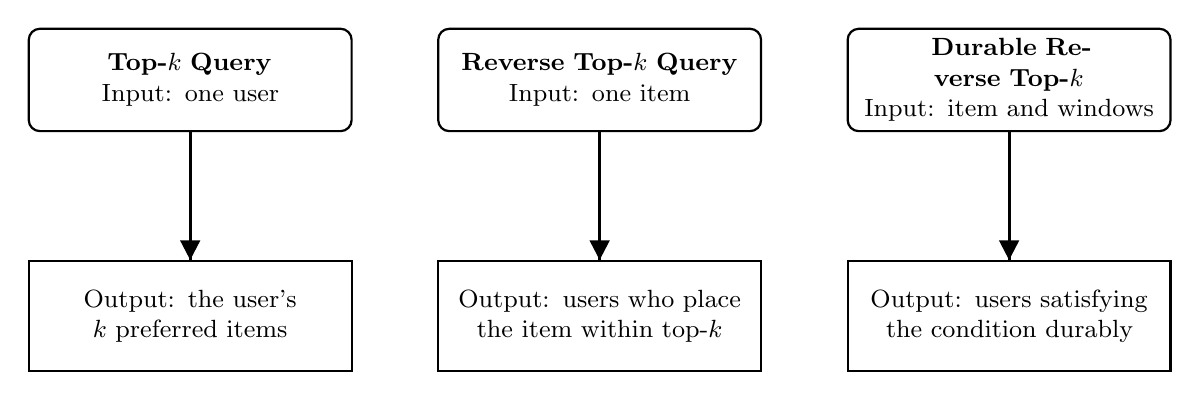
\begin{tikzpicture}[
font=\small,
querybox/.style={
rectangle,
rounded corners,
draw=black,
thick,
align=center,
minimum width=4.1cm,
minimum height=1.3cm,
text width=3.7cm
},
resultbox/.style={
rectangle,
draw=black,
thick,
align=center,
minimum width=4.1cm,
minimum height=1.4cm,
text width=3.7cm
}
]

\node[querybox] (topk) at (0,3)
{\textbf{Top-$k$ Query}\\Input: one user};

\node[resultbox] (topkresult) at (0,0)
{Output: the user's\\$k$ preferred items};

\node[querybox] (reverse) at (5.2,3)
{\textbf{Reverse Top-$k$ Query}\\Input: one item};

\node[resultbox] (reverseresult) at (5.2,0)
{Output: users who place\\the item within top-$k$};

\node[querybox] (durable) at (10.4,3)
{\textbf{Durable Reverse Top-$k$}\\Input: item and windows};

\node[resultbox] (durableresult) at (10.4,0)
{Output: users satisfying\\the condition durably};

% Arrow shafts (plain lines, no arrow-tip library required)
\draw[line width=1.1pt] (topk.south) -- (topkresult.north);
\draw[line width=1.1pt] (reverse.south) -- (reverseresult.north);
\draw[line width=1.1pt] (durable.south) -- (durableresult.north);

% Hand-drawn downward arrowheads (filled triangles, tip at the destination boundary)
\fill (topkresult.north) -- ++(0.13,0.25) -- ++(-0.26,0) -- cycle;
\fill (reverseresult.north) -- ++(0.13,0.25) -- ++(-0.26,0) -- cycle;
\fill (durableresult.north) -- ++(0.13,0.25) -- ++(-0.26,0) -- cycle;

\end{tikzpicture}
\caption{Conceptual comparison of top-$k$, reverse top-$k$, and durable reverse top-$k$ query processing}
\label{fig:query_comparison}
\end{figure}

Let $\mathcal{T}'\subseteq\mathcal{T}$ denote the set of temporal windows considered by a query, where

\begin{equation}
L'=\left|\mathcal{T}'\right|.
\label{eq:selected_window_count}
\end{equation}

Given a durability threshold $\tau\in(0,1]$, the minimum number of temporal windows in which the query item must satisfy the top-$k$ condition is

\begin{equation}
r=\left\lceil\tau L'\right\rceil.
\label{eq:durability_requirement}
\end{equation}

The durability count of user $u$ for query item $q$ is defined as

\begin{equation}
D(u,q,\mathcal{T}')
=
\sum_{t\in\mathcal{T}'}
\mathbb{I}
\left[
\operatorname{rank}(u,q,t)\leq k
\right],
\label{eq:durability_count}
\end{equation}

where $\mathbb{I}[\cdot]$ denotes the indicator function.

The durable reverse top-$k$ result set is defined as

\begin{equation}
\begin{aligned}
\operatorname{DRTop}\text{-}k(q,k,\tau,\mathcal{T}')
=
\bigl\{
u\in\mathcal{U}
\;\bigm|\;&
D(u,q,\mathcal{T}') \\
&\geq \left\lceil\tau L'\right\rceil
\bigr\}.
\end{aligned}
\label{eq:durable_reverse_topk}
\end{equation}

%----------------------------------------------------------------------------------------

\subsection{Problem Statement}
\label{subsec:problem_statement}

A straightforward exact solution evaluates every user in every selected temporal window and compares the query-item score with the scores of all available items. The approximate computational cost of this exhaustive verification is

\begin{equation}
O\left(nL'md\right),
\label{eq:exhaustive_complexity}
\end{equation}

where $n$ is the number of users, $L'$ is the number of selected temporal windows, $m$ is the number of items, and $d$ is the latent dimensionality. This cost becomes substantial for large recommendation datasets.

The central problem addressed in this thesis is stated as follows:

\begin{quote}
\textit{How can durable reverse top-$k$ users be identified efficiently over time-varying latent preferences without exhaustively verifying every user against every item in every temporal window?}
\end{quote}

The major challenges associated with the problem are summarized below:

\begin{itemize}

\item \textbf{Large search space:}
Exact verification may require evaluating thousands or millions of users against a large item collection.

\item \textbf{Multiple temporal windows:}
The top-$k$ condition must be evaluated repeatedly instead of being checked only once.

\item \textbf{Sparse interaction data:}
Some users may have limited or no ratings in particular temporal windows, making temporal preference construction difficult.

\item \textbf{Candidate-set selection:}
A very small candidate set reduces runtime but may exclude true durable users. A very large candidate set provides greater recall but reduces the computational benefit of filtering.

\item \textbf{Score-convention consistency:}
Dot-product preference scores follow a larger-is-better convention. Therefore, exact verification must compare the query-item score with the $k$-th largest score rather than the $k$-th smallest score.

\item \textbf{Accuracy--efficiency balance:}
The framework must provide substantial pruning and runtime improvement while maintaining high recall and precision.

\end{itemize}

To address these challenges, HyDART-RQ first applies the Durable Quantile Rank (DQR) filter to identify promising candidate users. Exact SSA or PRA verification is subsequently applied only to the filtered candidate set. The framework also supports an adaptive candidate budget so that the candidate-set size can be increased when a small fixed budget is likely to miss durable users.

The high-level workflow of HyDART-RQ is shown in Figure~\ref{fig:hydart_overview}.

\begin{figure}[H]
\centering
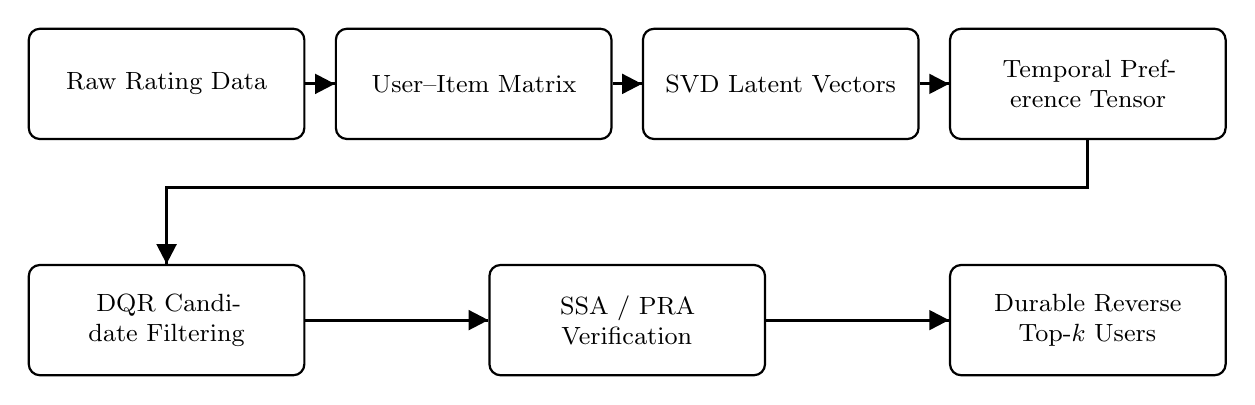
\begin{tikzpicture}[
font=\small,
stage/.style={
rectangle,
rounded corners,
draw=black,
thick,
align=center,
minimum width=3.5cm,
minimum height=1.4cm,
text width=3.2cm
}
]

\node[stage] (ratings) at (0,3)
{Raw Rating Data};

\node[stage] (matrix) at (3.9,3)
{User--Item Matrix};

\node[stage] (svd) at (7.8,3)
{SVD Latent Vectors};

\node[stage] (temporal) at (11.7,3)
{Temporal Preference Tensor};

\node[stage] (filter) at (0,0)
{DQR Candidate Filtering};

\node[stage] (verify) at (5.85,0)
{SSA / PRA Verification};

\node[stage] (result) at (11.7,0)
{Durable Reverse Top-$k$ Users};

% Arrow shafts (plain lines, no arrow-tip library required)
\draw[line width=1.1pt] (ratings.east) -- (matrix.west);
\draw[line width=1.1pt] (matrix.east) -- (svd.west);
\draw[line width=1.1pt] (svd.east) -- (temporal.west);
\draw[line width=1.1pt] (temporal.south) -- ++(0,-0.6) -| (filter.north);
\draw[line width=1.1pt] (filter.east) -- (verify.west);
\draw[line width=1.1pt] (verify.east) -- (result.west);

% Hand-drawn arrowheads (filled triangles, tip at the destination boundary)
\fill (matrix.west) -- ++(-0.25,0.13) -- ++(0,-0.26) -- cycle;
\fill (svd.west) -- ++(-0.25,0.13) -- ++(0,-0.26) -- cycle;
\fill (temporal.west) -- ++(-0.25,0.13) -- ++(0,-0.26) -- cycle;
\fill (filter.north) -- ++(0.13,0.25) -- ++(-0.26,0) -- cycle;
\fill (verify.west) -- ++(-0.25,0.13) -- ++(0,-0.26) -- cycle;
\fill (result.west) -- ++(-0.25,0.13) -- ++(0,-0.26) -- cycle;

\end{tikzpicture}
\caption{High-level workflow of the proposed HyDART-RQ framework}
\label{fig:hydart_overview}
\end{figure}

%----------------------------------------------------------------------------------------

\subsection{Motivating Example}
\label{subsec:motivating_example}

Consider a recommendation system containing five temporal windows. Let the query item be $q$, let $k=3$, and let the durability threshold be $\tau=0.6$. The minimum required number of successful windows is

\begin{equation}
\left\lceil\tau L\right\rceil
=
\left\lceil0.6\times5\right\rceil
=
3.
\label{eq:motivating_required_windows}
\end{equation}

Table~\ref{tab:motivating_example} presents the rank of query item $q$ for three users across five temporal windows.

\begin{table}[htbp]
\centering
\caption{Example of durable reverse top-$k$ qualification for $k=3$ and $\tau=0.6$}
\label{tab:motivating_example}
\small
\renewcommand{\arraystretch}{1.25}
\setlength{\tabcolsep}{5pt}
\begin{tabular}{|c|c|c|c|c|c|c|c|}
\hline
\textbf{User} &
\textbf{$t_1$} &
\textbf{$t_2$} &
\textbf{$t_3$} &
\textbf{$t_4$} &
\textbf{$t_5$} &
\textbf{Successful} &
\textbf{Durable} \\
\hline
$u_1$ & 2 & 3 & 5 & 2 & 3 & 4 & Yes \\
\hline
$u_2$ & 1 & 6 & 2 & 7 & 8 & 2 & No \\
\hline
$u_3$ & 4 & 2 & 3 & 5 & 1 & 3 & Yes \\
\hline
\end{tabular}
\end{table}

User $u_1$ ranks the query item within the top-$3$ in four windows and therefore satisfies the durability condition. User $u_2$ satisfies the top-$3$ condition in only two windows and is not durable. User $u_3$ satisfies the condition in exactly three windows and is therefore durable.

This example illustrates why a static reverse top-$k$ result can be misleading. If only the first temporal window were considered, user $u_2$ would appear highly relevant because the query item has rank $1$. However, the item does not remain highly ranked in the later windows. In contrast, user $u_3$ would be excluded in the first window even though the user satisfies the durability requirement over the complete interval.

For a large dataset, generating the complete rank sequence for every user requires extensive computation. HyDART-RQ therefore estimates which users are promising, eliminates unlikely users before exact verification, and retains a configurable number of candidates to preserve high result quality.

%----------------------------------------------------------------------------------------

\section{Objectives}
\label{sec:objectives}

The primary objective of this thesis is to develop an efficient hybrid framework for durable reverse top-$k$ query processing over time-varying preference data.

The specific objectives are as follows:

\begin{enumerate}

\item To formally define the durable reverse top-$k$ query problem using temporally varying latent user preferences.

\item To construct an end-to-end preprocessing pipeline that transforms timestamped rating data into sparse user--item matrices, latent item vectors, and temporal user-preference tensors.

\item To design and implement the Durable Quantile Rank (DQR) candidate filter for identifying users who are likely to satisfy the durability requirement.

\item To integrate the Sequential Search Algorithm (SSA) and the Pruning-based Algorithm (PRA) as exact durability verifiers within the HyDART-RQ framework.

\item To develop an adaptive candidate-budget mechanism that improves recall when a small fixed candidate set is insufficient.

\item To maintain consistency between the larger-is-better SVD scoring model and the ranking logic used by the filtering and verification components.

\item To evaluate the proposed framework using synthetic data and three real-world datasets: MovieLens, a subset of the Netflix Prize dataset, and Amazon Reviews 2023--Video Games.

\item To compare HyDART-RQ with full exact verification and alternative candidate-filtering strategies using recall, precision, exact-match ratio, pruning ratio, query-processing time, and speedup.

\item To investigate the sensitivity of the framework to parameters such as $k$, $\tau$, candidate factor $c$, latent dimension $d$, and number of temporal windows $L$.

\end{enumerate}

%----------------------------------------------------------------------------------------

\section{Scope}
\label{sec:scope}

The scope of this thesis is defined as follows:

\begin{itemize}

\item The research focuses on offline durable reverse top-$k$ queries over a predefined collection of query items.

\item User and item preferences are modeled using truncated SVD-based latent factors generated from sparse rating data.

\item Historical interactions are divided into equal-width temporal windows. The primary experiments use five windows, while sensitivity experiments examine alternative values.

\item The candidate-filtering methods include Durable Quantile Rank, Global Average, Union Window, and a legacy minimum-rank approach.

\item The DQR-based candidate filter forms the principal filtering component of HyDART-RQ.

\item SSA and PRA are used as exact durability verifiers for the selected candidate users.

\item Fixed and adaptive candidate-budget strategies are evaluated.

\item Experiments are conducted using synthetic data, MovieLens \texttt{ml\allowbreak-latest\allowbreak-small}, a selected Netflix Prize subset, and Amazon Reviews 2023--Video Games.

\item The framework is implemented in Python using NumPy, SciPy, pandas, and supporting scientific-computing libraries.

\item Evaluation is based on recall, precision, exact-match ratio, pruning ratio, average candidate count, query-processing time, and speedup.

\item Real-time streaming updates, distributed deployment, privacy-preserving recommendation, user-interface development, and causal analysis of user behaviour are outside the present scope.

\end{itemize}

Table~\ref{tab:scope_summary} summarizes the main boundaries of the study.

\begin{table}[htbp]
\centering
\caption{Summary of the research scope}
\label{tab:scope_summary}
\small
\renewcommand{\arraystretch}{1.25}
\setlength{\tabcolsep}{5pt}
\begin{tabularx}{\textwidth}{|p{3.3cm}|X|}
\hline
\textbf{Aspect} &
\textbf{Scope of the Thesis} \\
\hline
Query type &
Offline durable reverse top-$k$ query processing \\
\hline
Preference representation &
SVD-based latent user and item vectors \\
\hline
Temporal model &
Equal-width temporal windows and time-varying user vectors \\
\hline
Candidate filtering &
DQR, Global Average, Union Window, and legacy filtering \\
\hline
Exact verification &
Sequential Search Algorithm and Pruning-based Algorithm \\
\hline
Datasets &
Synthetic, MovieLens, Netflix Prize subset, and Amazon Video Games \\
\hline
Evaluation &
Recall, precision, pruning, exact matching, runtime, and speedup \\
\hline
Excluded areas &
Streaming updates, distributed execution, privacy-preserving processing, and user-interface design \\
\hline
\end{tabularx}
\end{table}

%----------------------------------------------------------------------------------------

\section{Unfamiliarity of the Problem, Topic, Solution}
\label{sec:unfamiliarity}

The proposed research is related to previous studies on reverse top-$k$ queries, approximate reverse ranking, temporal preference modeling, and durable query processing. However, HyDART-RQ is not a direct reproduction of any single existing approach. The originality of the work lies in the integration of durability-aware temporal rank filtering, exact candidate verification, adaptive candidate budgeting, and latent-factor recommendation within a unified processing framework.

The principal contributions are summarized in Table~\ref{tab:original_contributions}.

\begin{table}[htbp]
\centering
\caption{Original components and contributions of HyDART-RQ}
\label{tab:original_contributions}
\small
\renewcommand{\arraystretch}{1.25}
\setlength{\tabcolsep}{4pt}
\begin{tabularx}{\textwidth}{|p{3.5cm}|X|}
\hline
\textbf{Contribution} &
\textbf{Description} \\
\hline
Durable Quantile Rank filter &
Uses the temporal rank distribution of a query item to prioritize users who are more likely to satisfy the durability requirement. \\
\hline
Hybrid processing pipeline &
Combines approximate candidate filtering with exact SSA/PRA verification on a reduced user set. \\
\hline
Adaptive candidate budget &
Introduces a configurable minimum candidate count and boundary expansion to improve recall on sparse datasets. \\
\hline
Score-convention correction &
Ensures that all components consistently use the larger-is-better interpretation of SVD dot-product scores. \\
\hline
Unified data pipeline &
Processes synthetic, MovieLens, Netflix, and Amazon datasets through a common latent-factor and temporal-preference construction procedure. \\
\hline
Comprehensive evaluation &
Examines recall, precision, exact matching, pruning, runtime, speedup, scalability, and parameter sensitivity. \\
\hline
\end{tabularx}
\end{table}

The thesis does not claim that reverse top-$k$ queries, SVD, SSA, or PRA were independently invented in this work. These established concepts are acknowledged and adapted appropriately. The proposed contribution is the design and implementation of the complete HyDART-RQ framework and the investigation of how temporal candidate filtering and adaptive candidate selection can reduce the cost of exact durable reverse top-$k$ verification.

A particularly important contribution of the implementation is the identification and correction of a score-direction inconsistency. The original temporal verifiers used a smaller-is-better comparison, which is suitable for distance-based models. However, the SVD-based preference model used in this thesis produces dot-product similarity scores, for which larger values indicate stronger preferences. The verification condition was therefore corrected to compare the query-item score with the $k$-th largest item score. The corrected implementation was subsequently validated through correctness tests.

%----------------------------------------------------------------------------------------

\section{Project Planning}
\label{sec:project_planning}

The project was completed through a sequence of research, development, experimentation, validation, and documentation activities conducted over two academic semesters. Table~\ref{tab:project_plan} summarizes the major phases and their completion status.

\begin{table}[htbp]
\centering
\caption{Project planning and completion status}
\label{tab:project_plan}
\small
\renewcommand{\arraystretch}{1.25}
\setlength{\tabcolsep}{4pt}
\begin{tabularx}{\textwidth}{|p{1.0cm}|p{3.4cm}|X|p{2.0cm}|}
\hline
\textbf{Phase} &
\textbf{Activity} &
\textbf{Major Tasks} &
\textbf{Status} \\
\hline
1 &
Literature review &
Review of reverse top-$k$, approximate ranking, durable queries, and latent-factor recommendation &
Completed \\
\hline
2 &
Problem formulation &
Definition of temporal preferences, durability conditions, and evaluation requirements &
Completed \\
\hline
3 &
Data preparation &
Acquisition, cleaning, indexing, and temporal partitioning of datasets &
Completed \\
\hline
4 &
Baseline implementation &
Implementation and validation of full SSA, PRA, and static baselines &
Completed \\
\hline
5 &
Proposed framework &
Development of DQR filtering, hybrid processing, and adaptive candidate budgeting &
Completed \\
\hline
6 &
Experimentation &
Synthetic, MovieLens, Netflix, Amazon, robustness, and scalability experiments &
Completed \\
\hline
7 &
Testing and validation &
Correction of the score-direction inconsistency and execution of correctness tests &
Completed \\
\hline
8 &
Documentation &
Result analysis, figure preparation, and thesis writing &
Ongoing \\
\hline
\end{tabularx}
\end{table}

This thesis was completed as an individual capstone project. The author performed the literature review, problem formulation, data preparation, algorithm design, implementation, testing, experimentation, result analysis, visualization, and report preparation under the supervision of Dr.\ K.\ M.\ Azharul Hasan. The supervisor provided research guidance, technical suggestions, constructive feedback, and regular evaluation throughout the project.

%----------------------------------------------------------------------------------------

\section{Applications of the Work}
\label{sec:applications}

Durable reverse top-$k$ query processing has practical value in several application domains:

\begin{itemize}

\item \textbf{Targeted product promotion:}
E-commerce platforms can identify users who consistently rank a product or product category highly and direct promotional campaigns toward them.

\item \textbf{Audience discovery:}
Streaming platforms can identify users whose long-term preference profiles indicate sustained interest in a newly released movie, series, song, or game.

\item \textbf{Inventory planning:}
Retailers can estimate the durable audience of an item before adjusting stock levels or allocating promotional resources.

\item \textbf{Customer segmentation:}
Users can be separated into persistent-interest and temporary-interest groups according to the durability of their preferences.

\item \textbf{Gaming applications:}
Gaming platforms can identify players who consistently prefer related genres or franchises for beta testing, early access, or sequel promotion.

\item \textbf{Content and creator analysis:}
Social-media platforms can discover users who maintain sustained interest in particular creators, topics, or content categories.

\item \textbf{Long-term campaign evaluation:}
Marketing teams can distinguish short-term attention from durable user interest and prioritize audiences with more stable preferences.

\end{itemize}

Table~\ref{tab:application_summary} summarizes selected application scenarios.

\begin{table}[htbp]
\centering
\caption{Potential applications of durable reverse top-$k$ query processing}
\label{tab:application_summary}
\small
\renewcommand{\arraystretch}{1.25}
\setlength{\tabcolsep}{4pt}
\begin{tabularx}{\textwidth}{|p{3.2cm}|X|X|}
\hline
\textbf{Domain} &
\textbf{Query Item} &
\textbf{Possible Use} \\
\hline
E-commerce &
A product or product category &
Targeted promotion and inventory planning \\
\hline
Video streaming &
A movie, series, or genre &
Long-term audience discovery \\
\hline
Music streaming &
A song, artist, or music category &
Personalized campaign targeting \\
\hline
Gaming &
A game, franchise, or genre &
Beta-tester recruitment and sequel promotion \\
\hline
Social media &
A creator, topic, or content category &
Persistent audience identification \\
\hline
Market analysis &
A brand or product segment &
Distinguishing durable demand from temporary interest \\
\hline
\end{tabularx}
\end{table}

%----------------------------------------------------------------------------------------

\section{Organization of the Thesis}
\label{sec:thesis_organization}

This thesis is organized into seven chapters as follows:

\noindent
\textbf{Chapter I: Introduction.}
This chapter presents the research background, problem statement, motivating example, objectives, scope, originality, project planning, applications, and organization of the thesis.

\noindent
\textbf{Chapter II: Literature Review.}
This chapter reviews previous work related to reverse top-$k$ queries, approximate reverse ranking, durable query processing, temporal preferences, and matrix factorization. It also identifies the research gap addressed by HyDART-RQ.

\noindent
\textbf{Chapter III: Methodology.}
This chapter presents the complete HyDART-RQ methodology, including data preprocessing, latent-factor construction, temporal preference modeling, DQR filtering, SSA/PRA verification, and adaptive candidate budgeting.

\noindent
\textbf{Chapter IV: Implementation, Results and Discussions.}
This chapter describes the implementation environment, datasets, experimental settings, evaluation metrics, quantitative results, qualitative examples, and analysis of the proposed framework.

\noindent
\textbf{Chapter V: Societal, Health, Environment, Safety, Ethical, Legal and Cultural Issues.}
This chapter discusses intellectual-property considerations, dataset ethics, privacy, software licensing, sustainability, and the wider societal implications of the research.

\noindent
\textbf{Chapter VI: Addressing Complex Engineering Problems and Activities.}
This chapter explains the complex engineering problems associated with the project and the technical activities undertaken to design, implement, test, and validate the framework.

\noindent
\textbf{Chapter VII: Conclusions.}
This chapter summarizes the major findings and contributions, discusses the limitations of the current framework, and presents recommendations and future research directions.

%----------------------------------------------------------------------------------------
%	Chapter 2: Literature Review
%----------------------------------------------------------------------------------------
\chapter{Literature Review}
\label{ch:literature}

\section{Introduction}

This chapter surveys the body of work related to the Durable Reverse Top-$k$ (DRTop-$k$) problem. The relevant literature spans four interconnected research areas: (1) reverse top-$k$ query processing, (2) temporal and durable query processing, (3) collaborative filtering and matrix factorization, and (4) continuous monitoring of top-$k$ queries. For each area, we review the most significant contributions, identify their limitations, and situate them relative to our problem.

\section{Reverse Top-k Query Processing}

\subsection{Reverse Nearest Neighbour Queries}

The precursor to reverse top-$k$ queries is the \textit{reverse nearest neighbour (RNN)} query introduced by Korn and Muthukrishnan~\cite{korn2000influence}. An RNN query for a point $q$ in a metric space retrieves all data points that have $q$ as their nearest neighbour. Formally, the \textit{influence set} of $q$ is $\{p \in \mathcal{D} \mid \text{dist}(p, q) \leq \text{dist}(p, p') \text{ for all } p' \in \mathcal{D} \setminus \{p\}\}$. Applications include facility location, market analysis, and profile-based retrieval. The authors proposed exact and approximate algorithms based on pre-indexed Voronoi cells.

Subsequent work generalised RNN to reverse $k$-nearest neighbour (R$k$NN) queries~\cite{tao2004reverse}: find all objects that have $q$ as one of their $k$ nearest neighbours. These queries are still distance-based and assume a metric space, which does not directly model user preference rankings. Nevertheless, the conceptual duality---reversing the query direction---is foundational to our work.

\subsection{Reverse Top-k Queries}

Vlachou et al.~\cite{vlachou2010reverse} introduced the \textit{monochromatic and bichromatic reverse top-$k$} queries as a generalisation of RNN to preference-based settings. In their formulation, preferences are modeled as linear utility functions over a multidimensional attribute space. The reverse top-$k$ query for a product $q$ retrieves all customers $u$ such that $q$ is among $u$'s top-$k$ preferred products. The utility function $f_u(\mathbf{x}) = \sum_j w_{u,j} x_j$ assigns each customer $u$ a weight vector $\mathbf{w}_u$ over the product attributes $\mathbf{x}$.

Key contributions of~\cite{vlachou2010reverse} include:
\begin{itemize}
  \item An efficient algorithm exploiting the geometric structure of RT-$k$ regions in the weight vector space.
  \item Index structures (R-trees) for pruning non-qualifying customers.
  \item Distinction between monochromatic RT-$k$ (query from the same dataset) and bichromatic RT-$k$ (query item from a separate set).
\end{itemize}

Their setting, however, is entirely static: a single snapshot of customer weights is assumed. This does not accommodate the evolution of preferences over time.

Wu et al.~\cite{wu2009finch} proposed FINCH, an alternative approach to evaluating reverse top-$k$ queries using a pre-built index structure called the Fused Inverted and Containment Hierarchical index. FINCH supports efficient incremental updates and significantly outperforms scan-based methods for large datasets. However, like Vlachou et al., FINCH operates under a static preference model.

Vlachou et al.~\cite{vlachou2011monotone} extended reverse top-$k$ to monotone aggregate preference functions and proposed the VR-tree, a specialised index structure that prunes candidate customers based on dominance relationships. Again, the temporal dimension is absent.

\subsection{Probabilistic and Uncertain Reverse Top-k}

Lian and Chen~\cite{lian2010probabilistic} studied RT-$k$ queries over probabilistic databases, where attribute values are modeled as probability distributions. They introduced the concept of the reverse top-$k$ probability: $\Pr[q \in \text{top-}k(u)]$, and developed threshold-based algorithms to retrieve users whose RT-$k$ probability exceeds a given threshold. While this work incorporates uncertainty, it does not model the temporal evolution of preferences.

\section{Temporal Preference Modeling}

\subsection{Collaborative Filtering with Temporal Dynamics}

Koren~\cite{koren2009temporal} showed empirically that user preferences drift over time in the Netflix Prize dataset. He proposed \textit{TimeSVD++}, a matrix factorization model that parameterizes item biases and user biases as functions of time:
\[
  \hat{r}_{ui}(t) = \mu + b_i(t) + b_u(t) + \mathbf{p}_u(t)^\top \mathbf{q}_i
\]
where $b_u(t)$ and $\mathbf{p}_u(t)$ model the temporal drift in user biases and preferences. TimeSVD++ achieved state-of-the-art RMSE on the Netflix Prize benchmark. While this work demonstrates the importance of temporal preference modeling, it does not address any form of reverse top-$k$ query.

\subsection{Matrix Factorization for Recommendation}

Koren, Bell, and Volinsky~\cite{koren2009matrix} provided a comprehensive survey of matrix factorization techniques for recommender systems. Singular Value Decomposition (SVD) decomposes the rating matrix $R \approx U \Sigma V^\top$, where user and item latent vectors capture latent preference dimensions. Their regularized SVD (biased MF) model:
\[
  \hat{r}_{ui} = \mu + b_u + b_i + \mathbf{p}_u^\top \mathbf{q}_i
\]
is the backbone of modern recommendation systems and forms the basis for the preference scoring in our work.

Hu, Koren, and Volinsky~\cite{hu2008collaborative} extended MF to implicit feedback (clicks, views, purchases) using a weighted least-squares objective, where confidence weights $c_{ui} = 1 + \alpha r_{ui}$ amplify the signal from frequent interactions. This is particularly relevant for sparse datasets like Amazon Reviews.

Sarwar et al.~\cite{sarwar2001item} proposed item-based collaborative filtering as a scalable alternative to user-based CF, exploiting item--item similarity instead of user--user similarity. While predating modern MF methods, item-based CF remains a strong baseline for sparse datasets.

\section{Durable and Continuous Query Processing}

\subsection{Continuous Top-k Monitoring over Sliding Windows}

Mouratidis, Bakiras, and Papadias~\cite{mouratidis2006continuous} addressed the problem of continuously maintaining the top-$k$ result set as a sliding window of streaming data items moves. Their CATS algorithm uses cached partial results and incremental updates to avoid full re-evaluation of the top-$k$ on every window slide. Although this work targets top-$k$ (not reverse top-$k$) and a streaming setting (not offline temporal query processing), the concept of maintaining results across overlapping windows is related to the durability condition we impose.

\subsection{Durable Top-k Queries}

The notion of \textit{durability} in query results was formalised by Papapetrou and Pirrò~\cite{papapetrou2015durable}, who studied durable top-$k$ queries on temporal data. Their problem asks: over a timeline, find the objects that appear in the top-$k$ result for at least $\tau$ fraction of the time. They proposed a temporal index structure for efficient evaluation. The key difference from our work is the direction of the query: they retrieve items for a fixed user (top-$k$), whereas we retrieve users for a fixed item (reverse top-$k$). Adapting their index structures to the reverse direction is non-trivial because the candidate space is the set of users, not items.

\subsection{Sweep Sort Algorithm and Priority Region Algorithm}

The Sweep Sort Algorithm (SSA) \cite{mouratidis2006continuous} and Priority Region Algorithm (PRA) are temporal query processing techniques that operate on run-length encoded preference bitmaps. Given a bitmap $h[u][\cdot]$ where $h[u][t] = 1$ iff item $q$ ranks within top-$k$ for user $u$ at time $t$, the algorithms efficiently count the number of ``1'' runs (contiguous active windows) that overlap with a query interval $[t_b, t_e)$. The SSA performs a linear sweep over runs sorted by start time; the PRA builds a containment forest enabling DFS-based pruning of subtrees that cannot contribute sufficient duration. These algorithms serve as the \textit{verifiers} in our HyDART-RQ pipeline.

\section{Dataset Benchmarks}

\subsection{MovieLens Dataset}

Harper and Konstan~\cite{harper2016movielens} documented the history and design of the MovieLens datasets, which have been central benchmarks in collaborative filtering research since 1997. The MovieLens 100K dataset contains 100{,}000 ratings from 943 users on 1{,}682 movies, while larger variants (1M, 10M, 25M) are available. The ratings include explicit timestamps, making MovieLens suitable for temporal preference analysis. We use the ML-100K variant due to its tractable size for controlled experiments.

\subsection{Netflix Prize Dataset}

Bennett and Lanning~\cite{bennett2007netflix} described the Netflix Prize competition (2006--2009), which released 100 million anonymous movie ratings from approximately 480{,}000 subscribers on nearly 18{,}000 movies. The scale and temporal richness of this dataset have made it a standard benchmark for large-scale collaborative filtering. We use a 5{,}000-user, 3{,}000-item subset extracted by selecting the most active users and most-rated items.

\subsection{Amazon Reviews 2023}

The Amazon Reviews 2023 dataset~\cite{hou2024bridging} is a large-scale collection of product reviews across multiple categories. We use the Video Games category (5-core filtered), which contains approximately 94{,}762 interactions from 4{,}716 users on 2{,}996 items after applying our medium-subset extraction procedure. The dataset spans the years 2000--2023, providing a long temporal horizon for multi-window analysis.

\section{Research Gap Analysis}

Table~\ref{tab:litreview} summarizes the key dimensions of related work and identifies where our contribution sits.

\begin{table}[htbp]
\centering
\caption{Summary of Related Work and Research Gap}
\label{tab:litreview}
\footnotesize
\setlength{\tabcolsep}{3pt}
\begin{tabular}{lccccc}
\toprule
\textbf{Work} & \textbf{Query} & \textbf{Temporal} & \textbf{Durable} & \textbf{MF-based} & \textbf{Pruning} \\
\midrule
Korn \& Muthukrishnan~\cite{korn2000influence}    & Rev.\ NN        & \xmark & \xmark & \xmark & Voronoi \\
Vlachou et al.~\cite{vlachou2010reverse}           & Rev.\ Top-$k$   & \xmark & \xmark & \xmark & R-tree \\
Wu et al. (FINCH)~\cite{wu2009finch}               & Rev.\ Top-$k$   & \xmark & \xmark & \xmark & Index \\
Vlachou et al.~\cite{vlachou2011monotone}          & Rev.\ Top-$k$   & \xmark & \xmark & \xmark & Dominance \\
Lian \& Chen~\cite{lian2010probabilistic}          & Prob.\ RT-$k$   & \xmark & \xmark & \xmark & Threshold \\
Koren~\cite{koren2009temporal}                     & Top-$k$         & \cmark & \xmark & \cmark & None \\
Mouratidis et al.~\cite{mouratidis2006continuous}  & Top-$k$         & \cmark & \cmark & \xmark & Bitmap \\
Papapetrou \& Pirrò~\cite{papapetrou2015durable}   & Dur.\ Top-$k$   & \cmark & \cmark & \xmark & Temporal idx \\
\midrule
\textbf{HyDART-RQ (ours)}                          & Dur.\ Rev.\ Top-$k$ & \cmark & \cmark & \cmark & DQR filter \\
\bottomrule
\multicolumn{6}{l}{\xmark~=~not addressed, \cmark~=~addressed}
\end{tabular}
\end{table}

The table reveals a clear research gap: no existing work simultaneously addresses the reverse top-$k$ direction, temporal preference evolution, durability constraints, and matrix factorization-based preference modeling with a dedicated pruning strategy. Our HyDART-RQ framework fills precisely this gap.

\section{Discussion}

The existing literature provides important building blocks for our work: (1) the conceptual framework of reverse top-$k$ from~\cite{vlachou2010reverse}, (2) the temporal preference modeling via SVD from~\cite{koren2009matrix,koren2009temporal}, and (3) the SSA/PRA verifiers for bitmap-based durability checking inspired by~\cite{mouratidis2006continuous}. However, none of these threads have been combined into a single system targeting the DRTop-$k$ problem.

The primary challenge of integrating these components is the \textit{score convention mismatch}: static RT-$k$ and durable top-$k$ literature uses geometric/distance-based metrics (smaller is better), whereas SVD dot-product scores are similarity-based (larger is better). This mismatch, if undetected, leads to completely inverted results---returning users who dislike the query item rather than those who like it. We identify this bug, trace it to the original bitmap-construction logic, and correct it as part of this thesis.

\section{Chapter Summary}

This chapter reviewed the literature across four areas relevant to the DRTop-$k$ problem. Static RT-$k$ methods are efficient but ignore temporal dynamics. Temporal CF models (TimeSVD++) capture preference drift but do not support reverse queries. Durable query processing methods handle duration but target forward top-$k$, not reverse top-$k$. No existing work combines all four dimensions. The following chapter presents our HyDART-RQ methodology that bridges these gaps.

%----------------------------------------------------------------------------------------
%	Chapter 3: Methodology
%----------------------------------------------------------------------------------------
\chapter{Methodology}
\label{ch:methodology}

\section{Introduction}

This chapter presents the complete HyDART-RQ methodology, from formal problem definitions through the full algorithmic pipeline. Figure~\ref{fig:pipeline} shows the high-level architecture: raw rating data flows through SVD-based preprocessing to produce item embeddings $S$ and a temporal user tensor $W$; at query time, the DQR filter prunes the user space to a small candidate set, which is then exactly verified by the SSA or PRA verifier. We detail each component in the following sections.

\begin{figure}[htbp]
\centering
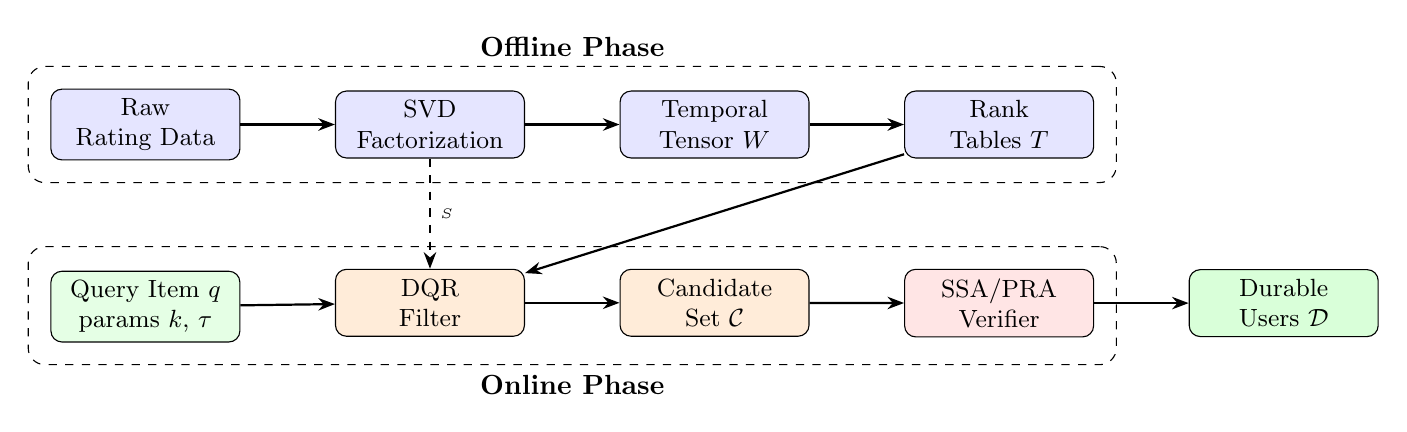
\begin{tikzpicture}[
  node distance=0.6cm and 1.2cm,
  box/.style={draw, rounded corners=4pt, minimum width=2.4cm, minimum height=0.85cm, align=center, font=\small},
  arrow/.style={-{Stealth[length=6pt]}, thick},
  phase/.style={draw, dashed, rounded corners=6pt, inner sep=8pt},
]

% Offline phase nodes
\node[box, fill=blue!10] (raw) {Raw\\Rating Data};
\node[box, fill=blue!10, right=of raw] (svd) {SVD\\Factorization};
\node[box, fill=blue!10, right=of svd] (tensor) {Temporal\\Tensor $W$};
\node[box, fill=blue!10, right=of tensor] (rtable) {Rank\\Tables $T$};

% Query time nodes
\node[box, fill=green!10, below=1.4cm of raw] (query) {Query Item $q$\\params $k$, $\tau$};
\node[box, fill=orange!15, below=1.4cm of svd] (dqr) {DQR\\Filter};
\node[box, fill=orange!15, below=1.4cm of tensor] (cand) {Candidate\\Set $\mathcal{C}$};
\node[box, fill=red!10, below=1.4cm of rtable] (ssa) {SSA/PRA\\Verifier};
\node[box, fill=green!15, right=1.2cm of ssa] (result) {Durable\\Users $\mathcal{D}$};

% Offline phase bracket
\node[phase, fit=(raw)(svd)(tensor)(rtable), label=above:{\textbf{Offline Phase}}] {};

% Online phase bracket
\node[phase, fit=(query)(dqr)(cand)(ssa), label=below:{\textbf{Online Phase}}] {};

% Arrows offline
\draw[arrow] (raw) -- (svd);
\draw[arrow] (svd) -- (tensor);
\draw[arrow] (tensor) -- (rtable);

% Arrows online
\draw[arrow] (query) -- (dqr);
\draw[arrow] (rtable) -- (dqr);
\draw[arrow] (dqr) -- (cand);
\draw[arrow] (cand) -- (ssa);
\draw[arrow] (ssa) -- (result);

% Cross-phase arrow
\draw[arrow, dashed] (svd) -- (dqr) node[midway, right, font=\tiny] {$S$};
\end{tikzpicture}
\caption{HyDART-RQ two-phase pipeline. The offline phase pre-computes factorizations and rank tables; the online phase applies DQR filtering followed by exact SSA/PRA verification.}
\label{fig:pipeline}
\end{figure}

\section{Notation and Problem Formalization}

Table~\ref{tab:notation} defines all symbols used throughout the thesis.

\begin{table}[htbp]
\centering
\caption{Summary of Notation}
\label{tab:notation}
\begin{tabular}{cl}
\toprule
\textbf{Symbol} & \textbf{Description} \\
\midrule
$\mathcal{U}$, $n_u$ & Set of users and its cardinality \\
$\mathcal{I}$, $n_i$ & Set of items and its cardinality \\
$R \in \mathbb{R}^{n_u \times n_i}$ & Sparse user-item rating matrix \\
$d$ & Latent factor dimensionality \\
$U \in \mathbb{R}^{n_u \times d}$ & User latent factor matrix (SVD) \\
$S \in \mathbb{R}^{n_i \times d}$ & Item latent factor matrix (SVD) \\
$L$ & Number of time windows \\
$W \in \mathbb{R}^{n_u \times L \times d}$ & Temporal user preference tensor \\
$\mathbf{w}_{u,t}$ & User $u$'s preference vector in window $t$ (row of $W$) \\
$\mathbf{s}_q$ & Item $q$'s latent vector (row of $S$) \\
$\text{score}(u, q, t)$ & Preference score: $\mathbf{w}_{u,t} \cdot \mathbf{s}_q$ \\
$\text{rank}(u, q, t)$ & Rank of item $q$ for user $u$ in window $t$ (1 = most preferred) \\
$k$ & Top-$k$ threshold \\
$\tau \in (0,1]$ & Durability threshold (fraction of windows) \\
$[t_b, t_e)$ & Query time interval \\
$L' = t_e - t_b$ & Number of windows in query interval \\
$\mathcal{D}(q, k, \tau)$ & Result set: durable reverse top-$k$ users \\
$c \geq 1$ & DQR relaxation factor \\
$T \in \mathbb{Z}^{n_u \times \tau_s}$ & Rank table (rank of each user's $\tau$-th quantile per window) \\
$\mathcal{C}$ & Candidate set output by DQR filter \\
$\tau_s$ & Number of quantile levels in rank table \\
\bottomrule
\end{tabular}
\end{table}

\noindent\textbf{Definition 1 (Preference Score):}
For user $u \in \mathcal{U}$, item $q \in \mathcal{I}$, and time window $t \in \{0, \ldots, L-1\}$, the preference score is:
\[
  \text{score}(u, q, t) = \mathbf{w}_{u,t} \cdot \mathbf{s}_q = \sum_{j=1}^{d} w_{u,t,j} \cdot s_{q,j}
\]
A \emph{higher} score indicates stronger preference (larger-is-better convention).

\medskip
\noindent\textbf{Definition 2 (Rank):}
$\text{rank}(u, q, t) = |\{i \in \mathcal{I} : \text{score}(u, i, t) \geq \text{score}(u, q, t)\}|$. Item $q$ is in $u$'s top-$k$ at time $t$ iff $\text{rank}(u, q, t) \leq k$.

\medskip
\noindent\textbf{Definition 3 (Durability):}
The durability of user $u$ with respect to query item $q$, threshold $k$, over interval $[t_b, t_e)$ is:
\[
  \text{dur}(u, q, k, [t_b, t_e)) = \frac{|\{t \in [t_b, t_e) : \text{rank}(u, q, t) \leq k\}|}{t_e - t_b}
\]

\medskip
\noindent\textbf{Definition 4 (DRTop-$k$ Query):}
$\text{DRTop-}k(q, k, \tau, [t_b, t_e)) = \{u \in \mathcal{U} : \text{dur}(u, q, k, [t_b, t_e)) \geq \tau\}$

\section{Offline Phase: Data Preprocessing}

\subsection{Rating Matrix Construction}

Given raw interaction records $(u_i, q_i, r_i, t_i)$ where $u_i$ is a user, $q_i$ is an item, $r_i$ is a numerical rating, and $t_i$ is a Unix timestamp, we first map users and items to integer indices $\{0, \ldots, n_u - 1\}$ and $\{0, \ldots, n_i - 1\}$ respectively using category encoding. The sparse rating matrix $R \in \mathbb{R}^{n_u \times n_i}$ is constructed with $R[u, i] = r_{u,i}$ for observed ratings and 0 elsewhere (stored in CSR format using \texttt{scipy.sparse.csr\_matrix}).

\subsection{SVD Factorization}

We apply truncated SVD to the sparse matrix $R$ using \texttt{scipy.sparse.linalg.svds}:
\[
  R \approx \hat{U} \Sigma \hat{V}^\top
\]
where $\hat{U} \in \mathbb{R}^{n_u \times d}$, $\Sigma \in \mathbb{R}^{d \times d}$ (diagonal), $\hat{V} \in \mathbb{R}^{n_i \times d}$, and $d$ is the latent dimensionality. The user matrix $U = \hat{U} \Sigma^{1/2}$ and item matrix $S = \hat{V} \Sigma^{1/2}$ are computed by absorbing the singular values symmetrically. Both $U$ and $S$ are then $\ell_2$-normalized along the latent dimension so that dot-products approximate cosine similarity. This normalization is critical for the rank table construction to be meaningful across users.

\subsection{Temporal User Preference Tensor Construction}

The historical time span $[T_{\min}, T_{\max}]$ is divided into $L$ equal-width windows using \texttt{numpy.linspace}. For window $t$, the boundaries are $[T_t, T_{t+1})$. The temporal tensor $W \in \mathbb{R}^{n_u \times L \times d}$ is initialized to zero. For each rating $(u, i, r, t_{\text{unix}})$, we identify the window index $t = \lfloor L \cdot (t_{\text{unix}} - T_{\min}) / (T_{\max} - T_{\min}) \rfloor$ and accumulate the item latent vector:
\[
  W[u, t] \mathrel{+}= S[i]
\]
using \texttt{numpy.add.at} to correctly handle repeated $(u, t)$ indices. After accumulation, each $W[u, t]$ is divided by the number of items user $u$ rated in window $t$ to produce the average. Windows with no interactions fall back to the previous window's preference vector, or to the user's global average if all windows are empty.

Figure~\ref{fig:windows} illustrates the temporal window construction.

\begin{figure}[htbp]
\centering
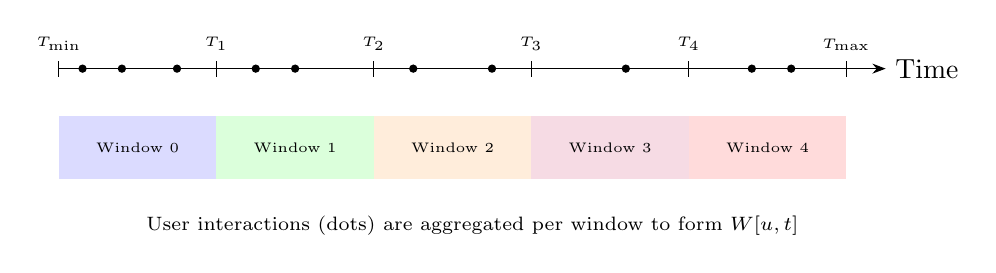
\begin{tikzpicture}[scale=1.0]
  % Timeline
  \draw[-{Stealth}] (0,0) -- (10.5,0) node[right] {Time};
  \foreach \x/\lab in {0/$T_{\min}$, 2/$T_1$, 4/$T_2$, 6/$T_3$, 8/$T_4$, 10/$T_{\max}$} {
    \draw (\x, -0.1) -- (\x, 0.1) node[above, font=\tiny] {\lab};
  }
  % Windows
  \foreach \x/\c/\l in {0/blue!20/Window 0, 2/green!20/Window 1, 4/orange!20/Window 2, 6/purple!20/Window 3, 8/red!20/Window 4} {
    \fill[\c, opacity=0.7] (\x, -0.6) rectangle (\x+2, -1.4);
    \node[font=\tiny] at (\x+1, -1.0) {\l};
  }
  % Ratings (dots)
  \foreach \xp/\yu in {0.3/u_1, 0.8/u_2, 1.5/u_1, 2.5/u_3, 3.0/u_1, 4.5/u_2, 5.5/u_3, 7.2/u_1, 8.8/u_2, 9.3/u_1} {
    \fill[black] (\xp, 0) circle (1.5pt);
  }
  \node[font=\scriptsize] at (5.25, -2.0) {User interactions (dots) are aggregated per window to form $W[u, t]$};
\end{tikzpicture}
\caption{Temporal window construction. The time axis $[T_{\min}, T_{\max}]$ is divided into $L=5$ equal windows. User interactions within each window are averaged to produce $\mathbf{w}_{u,t}$.}
\label{fig:windows}
\end{figure}

\section{Rank Table Construction}

Computing $\text{rank}(u, q, t)$ exactly requires scoring all $n_i$ items for user $u$ at time $t$ and sorting---an $O(n_i)$ operation per (user, window) pair. For a candidate filter, we need a fast approximation.

We pre-compute a \textit{rank table} $T \in \mathbb{R}^{n_u \times \tau_s}$ where $T[u, \ell]$ is the $\ell$-th largest preference score user $u$ assigns across all items in a single time window $t^*$ (typically the most recent window or a representative snapshot). The table is constructed using \texttt{numpy.partition} for efficiency:
\begin{enumerate}
  \item Compute all item scores for window $t^*$: $\text{scores}[u] = W[u, t^*] S^\top \in \mathbb{R}^{n_i}$.
  \item Partition and sort to obtain the top-$\tau_s$ scores in decreasing order for each user.
  \item Store as $T[u, :] = \text{sorted top-}\tau_s\text{ scores for user }u$.
\end{enumerate}

A companion table $\text{THR}[u, k-1]$ stores the $k$-th largest score (the boundary score for top-$k$ membership). Given a query item $q$ with score $\text{score}(u, q, t)$ at time $t$, we estimate the rank of $q$ for user $u$ using binary search on $T[u, :]$:
\[
  \hat{r}(u, q, t) = \text{searchsorted}(T[u], \text{score}(u, q, t), \text{side}=\text{'right'})
\]
This runs in $O(\log \tau_s)$ and provides a lower bound on the true rank.

\section{DQR Candidate Filter}

\subsection{Motivation}

For a given query item $q$, users with very low preference scores for $q$ in most windows cannot possibly achieve durability $\geq \tau$. The DQR filter formalizes this intuition.

\subsection{Durable Quantile Rank Definition}

Let $\hat{r}(u, q, t)$ denote the estimated rank of item $q$ for user $u$ in window $t$ (computed from rank tables). Define the \textit{Durable Quantile Rank} of user $u$ with respect to query $q$ as:
\[
  \text{DQR}(u, q) = \hat{r}(u, q)_{(\lceil \tau \cdot L \rceil)}
\]
where $\hat{r}(u, q)_{(j)}$ denotes the $j$-th smallest rank estimate among all $L$ windows (i.e., the $\lceil \tau L \rceil$-th order statistic of the rank estimates). Intuitively, $\text{DQR}(u, q)$ is the rank that $q$ must achieve in the ``best'' $\lceil \tau L \rceil$ windows for user $u$ to be durable.

\subsection{Pruning Rule}

A user $u$ can \emph{only} be durable if $\text{DQR}(u, q) \leq k$. We relax this to $\text{DQR}(u, q) \leq c \cdot k$ (with $c \geq 1$) to compensate for rank estimation error and retain all true results with high probability. The candidate set is:
\[
  \mathcal{C} = \{u \in \mathcal{U} : \text{DQR}(u, q) \leq c \cdot k\}
\]

In practice, we sort users by their DQR score and select the top-$M$ (where $M = \lceil c \cdot k \rceil$ or an adaptive budget; see Section~\ref{sec:adaptive}).

\subsection{DQR Filter Algorithm}

Algorithm~\ref{alg:dqr} presents the DQR candidate filter.

\begin{algorithm}[htbp]
\SetAlgoLined
\KwIn{Score matrix $\mathbf{F} \in \mathbb{R}^{n_u \times L}$ where $F[u,t] = \mathbf{w}_{u,t} \cdot \mathbf{s}_q$; durability $\tau$; relaxation $c$; threshold $k$; rank tables $T$}
\KwOut{Candidate set $\mathcal{C}$}

$r\_\text{req} \leftarrow \lceil \tau \cdot L \rceil$ \tcp{number of windows that must satisfy top-$k$}
$M \leftarrow \lceil c \cdot k \rceil$ \tcp{maximum candidate rank}
$\text{dqr}[\,] \leftarrow \infty$ \tcp{DQR scores for all users}

\For{each user $u \in \{0, \ldots, n_u - 1\}$}{
  \For{each window $t \in \{0, \ldots, L-1\}$}{
    $\hat{r}_{u,t} \leftarrow \text{searchsorted}(T[u], F[u,t], \text{side=right})$ \tcp{estimated rank}
  }
  Sort $\{\hat{r}_{u,0}, \ldots, \hat{r}_{u,L-1}\}$ in ascending order\;
  $\text{dqr}[u] \leftarrow \hat{r}_{u, r\_\text{req} - 1}$ \tcp{$r\_\text{req}$-th smallest rank}
}
$\mathcal{C} \leftarrow \{u : \text{dqr}[u] \leq M\}$\;
\Return $\mathcal{C}$
\caption{DQR Candidate Filter}
\label{alg:dqr}
\end{algorithm}

The time complexity of the DQR filter is $O(n_u \cdot L \cdot \log \tau_s + n_u \cdot L \log L)$, dominated by the binary-search rank estimation step and the per-user sort over $L$ windows. Since $L$ and $\tau_s$ are small constants (typically 5 and 500), this reduces to $O(n_u)$ in practice.

\section{Exact Verifiers: SSA and PRA}

\subsection{Bitmap Construction}

For each candidate user $u \in \mathcal{C}$, we compute the exact preference bitmap $h[u] \in \{0,1\}^L$:
\[
  h[u][t] = \begin{cases} 1 & \text{if } \text{rank}(u, q, t) \leq k \\ 0 & \text{otherwise} \end{cases}
\]
Computing $\text{rank}(u, q, t)$ exactly requires scoring all $n_i$ items for user $u$ in window $t$ to find the $k$-th largest score, then comparing $\text{score}(u, q, t)$ against it. This is done in a vectorized manner for all candidates simultaneously:
\begin{enumerate}
  \item For each window $t$: compute $\text{scores}[t] = W[\mathcal{C}, t] \cdot S^\top \in \mathbb{R}^{|\mathcal{C}| \times n_i}$.
  \item Partition columns: $\text{kth}[t] = \text{scores}[t]_{(:, n_i - k)}$ (the $k$-th largest value per candidate).
  \item $h[u][t] = 1$ if $\text{scores}[t][u, q] \geq \text{kth}[t][u]$, else 0.
\end{enumerate}

Bitmap values are then run-length encoded into a list of runs (start, end) where $h[u][t] = 1$ for all $t \in [\text{start}, \text{end})$.

\subsection{Sweep Sort Algorithm (SSA)}

Algorithm~\ref{alg:ssa} presents the SSA verifier.

\begin{algorithm}[htbp]
\SetAlgoLined
\KwIn{Run-length encoded bitmap \texttt{runs}$[u]$ for each candidate $u \in \mathcal{C}$; query interval $[t_b, t_e)$; durability $\tau$}
\KwOut{Durable users $\mathcal{D}$}
$\text{req} \leftarrow \lceil \tau \cdot (t_e - t_b) \rceil$ \tcp{required active windows}
$\mathcal{D} \leftarrow \emptyset$\;

\For{each user $u \in \mathcal{C}$}{
  $\text{count} \leftarrow 0$\;
  \For{each run $(s, e)$ in \texttt{runs}$[u]$ sorted by $s$}{
    $\text{overlap} \leftarrow \min(e, t_e) - \max(s, t_b)$\;
    \If{$\text{overlap} > 0$}{$\text{count} \leftarrow \text{count} + \text{overlap}$}
  }
  \If{$\text{count} \geq \text{req}$}{$\mathcal{D} \leftarrow \mathcal{D} \cup \{u\}$}
}
\Return $\mathcal{D}$
\caption{Sweep Sort Algorithm (SSA) Verifier}
\label{alg:ssa}
\end{algorithm}

The SSA verifier runs in $O(|\mathcal{C}| \cdot n_{\text{runs}})$ where $n_{\text{runs}}$ is the average number of runs per user, which is bounded by $L$.

\subsection{Priority Region Algorithm (PRA)}

The PRA builds a forest of containment trees over the bitmap runs, where a run $[s_1, e_1)$ is a parent of $[s_2, e_2)$ if $[s_2, e_2) \subseteq [s_1, e_1)$. For a query $[t_b, t_e)$, DFS traversal over the forest allows early pruning: if the maximum possible overlap of a subtree with $[t_b, t_e)$ plus the already-accumulated count is less than $\text{req}$, the entire subtree is pruned.

In practice, for $L = 5$, the PRA and SSA achieve similar performance (the forest depth is at most $L$). For larger $L$, PRA yields greater pruning benefit.

\section{HyDART-RQ: The Hybrid Pipeline}
\label{sec:hydart}

Algorithm~\ref{alg:hydart} presents the complete HyDART-RQ pipeline.

\begin{algorithm}[htbp]
\SetAlgoLined
\KwIn{$S$ (item matrix), $W$ (user tensor), query item $q$, params $k, \tau, c, [t_b, t_e)$, rank tables $T$}
\KwOut{Durable users $\mathcal{D}$}
\textbf{Phase 1: DQR Filtering}\\
Compute score matrix $F[u, t] \leftarrow \mathbf{w}_{u,t} \cdot \mathbf{s}_q$ for all $u, t$\;
$\mathcal{C} \leftarrow \text{DQR-Filter}(F, T, \tau, c, k)$ \tcp{Algorithm~\ref{alg:dqr}}

\BlankLine
\textbf{Phase 2: Exact Verification}\\
Extract candidate tensor $W_\mathcal{C} \leftarrow W[\mathcal{C}, :, :]$\;
\For{each window $t \in [t_b, t_e)$}{
  $\text{all\_scores}[t] \leftarrow W_\mathcal{C}[:,t,:] \cdot S^\top$ \tcp{shape $|\mathcal{C}| \times n_i$}
  $\text{kth}[t] \leftarrow$ $k$-th largest column value per row\;
  $h[:, t] \leftarrow (\text{all\_scores}[t][:, q] \geq \text{kth}[t])$
}
Encode $h$ into run-length representations \texttt{runs}\;
$\mathcal{D} \leftarrow \text{SSA-Verify}(\text{runs}, [t_b, t_e), \tau)$ \tcp{Algorithm~\ref{alg:ssa}}

\Return $\mathcal{D}$
\caption{HyDART-RQ: Hybrid Durable Approximate Reverse Top-$k$ Query}
\label{alg:hydart}
\end{algorithm}

\subsection{Score Convention Correctness}

A critical implementation requirement is that preference scores are \emph{larger-is-better}: a higher dot-product score $\mathbf{w}_{u,t} \cdot \mathbf{s}_q$ means user $u$ prefers item $q$ more strongly in window $t$. Consequently:
\begin{itemize}
  \item Top-$k$ membership: $q \in \text{top-}k(u, t)$ iff $\text{score}(u, q, t) \geq \text{score}(u, i_{(k)}, t)$ where $i_{(k)}$ is the $k$-th ranked item.
  \item Bitmap: $h[u][t] = 1$ iff $\text{score}(u, q, t) \geq \text{kth-largest score for user }u\text{ in window }t$.
  \item DQR estimation: rank is estimated as the number of items with scores \emph{greater than or equal} to $\text{score}(u, q, t)$.
\end{itemize}

An earlier implementation had the comparison inverted (``$\leq$ kth-smallest score''---a smaller-is-better convention appropriate for distance-based metrics). This caused the bitmap to flag windows where $q$ was least preferred, and the result set contained users who \emph{disliked} the query item. The correction was validated by eight unit tests covering edge cases (all windows active, no windows active, partial durability, tie-breaking). All tests pass after the fix.

\section{Adaptive Candidate Budget}
\label{sec:adaptive}

On sparse datasets (e.g., Netflix with highly unequal interaction distributions), the fixed threshold $M = \lceil c \cdot k \rceil$ may yield a candidate set that is too small and misses some true durable users. We introduce an \textit{adaptive} extension:

\begin{enumerate}
  \item Sort all users by DQR score in ascending order.
  \item Select the top-$\max(M, M_{\min})$ users, where $M_{\min}$ is a minimum budget hyperparameter (e.g., 200).
  \item Optionally, add users within a \textit{boundary margin}: users whose DQR score is within $\delta$ of the $M$-th user's DQR score.
\end{enumerate}

This guarantees that even if the DQR estimates are noisy, a sufficient number of candidates enter the verification phase. The trade-off is a modest increase in candidate set size and verification time.

\section{Complexity Analysis}

Table~\ref{tab:complexity} summarizes the time complexity of each component.

\begin{table}[htbp]
\centering
\caption{Time Complexity Analysis}
\label{tab:complexity}
\begin{tabular}{lll}
\toprule
\textbf{Component} & \textbf{Per-Query Complexity} & \textbf{Dominant Term} \\
\midrule
Rank table lookup (DQR) & $O(n_u \cdot L \cdot \log \tau_s)$ & $O(n_u)$ for fixed $L, \tau_s$ \\
DQR sort per user & $O(n_u \cdot L \log L)$ & $O(n_u)$ for fixed $L$ \\
Bitmap construction & $O(|\mathcal{C}| \cdot n_i)$ & $O(|\mathcal{C}| \cdot n_i)$ \\
SSA verification & $O(|\mathcal{C}| \cdot L)$ & $O(|\mathcal{C}|)$ for fixed $L$ \\
\midrule
\textbf{Total HyDART-RQ} & $O(n_u + |\mathcal{C}| \cdot n_i)$ & $O(|\mathcal{C}| \cdot n_i)$ \\
\textbf{Brute-Force SSA} & $O(n_u \cdot n_i)$ & $O(n_u \cdot n_i)$ \\
\bottomrule
\end{tabular}
\end{table}

Since $|\mathcal{C}| \ll n_u$ (pruning ratio $> 96\%$ in all experiments), HyDART-RQ achieves a speedup of approximately $n_u / |\mathcal{C}|$ over brute force, matching the observed 20--22$\times$ speedups in experiments.

\section{Offline Pre-computation}

The rank tables $T$ and the SVD factorization $S, U$ are computed once offline and stored as \texttt{.npy} binary files. For the three datasets, offline pre-computation takes between 30 seconds and 15 minutes depending on dataset size. All subsequent queries use the cached artifacts, making the online phase highly efficient.

\section{Chapter Summary}

This chapter presented the HyDART-RQ methodology in full detail. The key algorithmic innovation is the DQR filter, which reduces the per-query workload from $O(n_u \cdot n_i)$ to $O(|\mathcal{C}| \cdot n_i)$ by leveraging pre-computed rank tables to cheaply estimate user durability. The exact SSA/PRA verifiers ensure that surviving candidates are correctly classified as durable or non-durable. The score convention correction is essential for correctness. The following chapter presents the experimental evaluation of this pipeline.

%----------------------------------------------------------------------------------------
%	Chapter 4: Implementation, Results and Discussions
%----------------------------------------------------------------------------------------
\chapter{Implementation, Results and Discussions}
\label{ch:results}

\section{Introduction}

This chapter presents the implementation details of the HyDART-RQ framework, the experimental setup, the evaluation metrics, and the results across all three datasets. We compare HyDART-RQ against multiple baseline methods and conduct ablation studies to assess the contribution of individual design choices.

\section{Implementation}

The HyDART-RQ framework is implemented entirely in Python 3.12. The key libraries used are:
\begin{itemize}
  \item \textbf{NumPy 1.x}: Vectorised operations, tensor construction (\texttt{numpy.add.at}), partition-based top-$k$ selection.
  \item \textbf{SciPy}: Sparse matrix construction (\texttt{scipy.sparse.csr\_matrix}), truncated SVD (\texttt{scipy.sparse.linalg.svds}).
  \item \textbf{pandas}: Data loading, timestamp parsing, categorical encoding.
  \item \textbf{scikit-learn}: Data partitioning utilities.
  \item \textbf{huggingface\_hub}: Direct access to Amazon Reviews 2023 dataset files.
\end{itemize}

The project is organized as:
\begin{itemize}
  \item \texttt{data/common\_data.py}: Dataset loading and preprocessing functions.
  \item \texttt{baselines/durable/ssa.py}: SSA implementation.
  \item \texttt{baselines/durable/pra.py}: PRA implementation.
  \item \texttt{hybrid/candidate\_filter.py}: DQR and adaptive filter.
  \item \texttt{hybrid/durable\_verifier.py}: Verification on candidate set.
  \item \texttt{utils/rank\_table.py}: Rank table construction.
  \item \texttt{experiments/}: Per-dataset experiment scripts.
  \item \texttt{outputs/}: Experiment results in CSV and TXT format.
\end{itemize}

\subsection{Correctness Validation}

Before benchmarking, we ran eight unit tests comparing HyDART-RQ output against brute-force ground truth on synthetic data with known answers:
\begin{enumerate}
  \item All windows active for all users (durability = 1.0 for all).
  \item No windows active (empty result expected).
  \item Exactly $\tau$-fraction of windows active (boundary case).
  \item One user durable, all others not.
  \item Query item at rank 1 in all windows.
  \item Query item at rank $k+1$ in all windows (no durable users).
  \item Ties in preference scores.
  \item Partial query interval $[t_b, t_e) \subsetneq [0, L)$.
\end{enumerate}
All eight tests pass after the score-convention correction (see Section~\ref{sec:hydart}).

\section{Experimental Setup}

\subsection{Datasets}

Table~\ref{tab:datasets} summarises the three datasets used in evaluation.

\begin{table}[htbp]
\centering
\caption{Dataset Statistics}
\label{tab:datasets}
\begin{tabular}{lrrrrr}
\toprule
\textbf{Dataset} & \textbf{Users} & \textbf{Items} & \textbf{Ratings} & \textbf{Density (\%)} & \textbf{Year Range} \\
\midrule
MovieLens 100K  &    610 &  9{,}724 &   100{,}836 & 1.70  & 1996--2018 \\
Netflix (subset)& 5{,}000 &  3{,}000 & 1{,}097{,}628 & 7.32 & 2000--2005 \\
Amazon VG (subset)& 4{,}716 &  2{,}996 &    94{,}762 & 0.67  & 2000--2023 \\
\bottomrule
\end{tabular}
\end{table}

\begin{itemize}
  \item \textbf{MovieLens 100K}~\cite{harper2016movielens}: Explicit star ratings (0.5--5.0) on movies. Relatively dense and well-studied; used for baseline validation.
  \item \textbf{Netflix Prize (subset)}~\cite{bennett2007netflix}: Integer ratings (1--5) on movies. Denser than Amazon; high temporal concentration in 2004--2005. The 5{,}000-user, 3{,}000-item subset was selected by taking the most active users and most-rated items.
  \item \textbf{Amazon Reviews 2023 -- Video Games}~\cite{hou2024bridging}: Integer ratings (1--5) on video game products. Sparse and long time horizon (23 years). Downloaded from HuggingFace using \texttt{HfFileSystem}; 5-core filtered.
\end{itemize}

\subsection{Experimental Parameters}

Table~\ref{tab:params} shows the default parameter settings used in all experiments.

\begin{table}[htbp]
\centering
\caption{Default Experimental Parameters}
\label{tab:params}
\begin{tabular}{lll}
\toprule
\textbf{Parameter} & \textbf{Symbol} & \textbf{Default Value} \\
\midrule
Latent dimensionality & $d$       & 32 \\
Top-$k$ threshold     & $k$       & 10 \\
Durability threshold  & $\tau$    & 0.6 \\
DQR relaxation factor & $c$       & 2.0 (Netflix: 1.5 Amazon) \\
Time windows          & $L$       & 5 \\
Number of query items & $N_q$     & 50 (MovieLens), 50 (Netflix), 100 (Amazon) \\
Chunk size (SVD chunk)& --        & 500 \\
Rank table size       & $\tau_s$  & 500 \\
Random seed           & --        & 42 \\
\bottomrule
\end{tabular}
\end{table}

\subsection{Evaluated Methods}

\begin{itemize}
  \item \textbf{Full\_SSA}: Brute-force SSA on all users; used as ground-truth reference and timing baseline.
  \item \textbf{Full\_PRA}: Brute-force PRA on all users; alternative ground-truth baseline.
  \item \textbf{Hybrid\_SSA\_DurableRank (HyDART-RQ)}: DQR filter + SSA verifier (our main method).
  \item \textbf{Hybrid\_PRA\_DurableRank}: DQR filter + PRA verifier (variant of our method).
  \item \textbf{Hybrid\_SSA\_GlobalAvg}: DQR filter using global user average instead of temporal tensor.
  \item \textbf{Hybrid\_SSA\_UnionWin}: DQR filter using union of all windows for candidate selection.
  \item \textbf{Hybrid\_SSA\_LegacyMinRank}: DQR filter with the incorrect (inverted) score convention; included to quantify the impact of the bug.
\end{itemize}

\subsection{Evaluation Metrics}

\begin{itemize}
  \item \textbf{Recall}: $|\mathcal{D} \cap \mathcal{D}^*| / |\mathcal{D}^*|$ where $\mathcal{D}^*$ is the ground-truth result set. Measures the fraction of true durable users retrieved.
  \item \textbf{Precision}: $|\mathcal{D} \cap \mathcal{D}^*| / |\mathcal{D}|$. Measures the fraction of retrieved users that are truly durable.
  \item \textbf{Exact Match}: Fraction of query items for which $\mathcal{D} = \mathcal{D}^*$ exactly.
  \item \textbf{Pruning Ratio}: $1 - |\mathcal{C}| / n_u$. Fraction of users eliminated by the DQR filter.
  \item \textbf{Speedup}: $T_{\text{Full\_SSA}} / T_{\text{method}}$. How much faster the method is relative to brute force.
  \item \textbf{Query Time}: Average wall-clock time per query item (seconds).
\end{itemize}

\section{Results: MovieLens Dataset}

Table~\ref{tab:movielens_results} presents results on the MovieLens dataset.

\begin{table}[htbp]
\centering
\caption{Results on MovieLens 100K ($n_u=610$, $n_i=9{,}724$, $k=10$, $\tau=0.6$, $L=5$, 50 queries)}
\label{tab:movielens_results}
\begin{tabular}{lccccc}
\toprule
\textbf{Method} & \textbf{Time (s)} & \textbf{Recall} & \textbf{Precision} & \textbf{Pruning} & \textbf{Speedup} \\
\midrule
Full\_SSA           & 0.0131 & --    & --    & --     & 1.00$\times$ \\
Full\_PRA           & 0.0132 & --    & --    & --     & --  \\
Hybrid\_SSA\_GlobalAvg  & 0.0148 & 1.000 & 1.000 & 96.7\% & 0.89$\times$ \\
Hybrid\_SSA\_UnionWin   & 0.0162 & 1.000 & 1.000 & 92.1\% & 0.81$\times$ \\
\textbf{HyDART-RQ (SSA\_DurableRank)} & \textbf{0.0142} & \textbf{1.000} & \textbf{1.000} & \textbf{96.7\%} & \textbf{0.92$\times$} \\
Hybrid\_PRA\_DurableRank & 0.0145 & 1.000 & 1.000 & 96.7\% & 0.90$\times$ \\
LegacyMinRank (buggy) & 0.0355 & 0.000 & 0.000 & 96.7\% & 0.37$\times$ \\
\bottomrule
\end{tabular}
\end{table}

\textbf{Observations:}
\begin{itemize}
  \item HyDART-RQ achieves \textbf{perfect recall (1.00)} with \textbf{96.7\% pruning}, confirming that the DQR filter eliminates no true durable users.
  \item Due to the small user base ($n_u = 610$), the brute-force SSA runs in 13ms; the overhead of the DQR filter brings HyDART-RQ's time to 14ms, yielding a slight apparent slowdown vs.\ brute force. This is expected: the DQR filter amortizes at larger scale.
  \item \textbf{LegacyMinRank} (the inverted score convention) yields 0\% recall, demonstrating the severity of the score-convention bug---it returns exactly the users who \emph{least} prefer the query item.
  \item The GlobalAvg and UnionWin baselines also achieve perfect recall on MovieLens, indicating that even simpler candidate selection strategies work on dense, small-scale data.
\end{itemize}

\section{Results: Netflix Dataset}

The Netflix subset ($n_u = 5{,}000$, $n_i = 3{,}000$) provides a medium-scale evaluation with higher interaction density.

\subsection{Vanilla HyDART-RQ}

\begin{table}[htbp]
\centering
\caption{Results on Netflix Subset --- Vanilla Parameters ($c=1.5$, no adaptive budget, 50 queries)}
\label{tab:netflix_vanilla}
\begin{tabular}{lccccc}
\toprule
\textbf{Method} & \textbf{Time (s)} & \textbf{Recall} & \textbf{Precision} & \textbf{Pruning} & \textbf{Speedup} \\
\midrule
Full\_SSA             & 0.576  & --    & --    & --     & 1.00$\times$ \\
Full\_PRA             & 0.579  & --    & --    & --     & -- \\
Hybrid\_SSA\_GlobalAvg   & 0.0089 & 0.712 & 0.998 & 99.6\% & 64.7$\times$ \\
Hybrid\_SSA\_UnionWin    & 0.0298 & 0.891 & 1.000 & 98.8\% & 19.3$\times$ \\
\textbf{HyDART-RQ (vanilla, $c=1.5$)} & 0.0268 & 0.554 & 1.000 & 99.6\% & 21.5$\times$ \\
Hybrid\_PRA\_DurableRank & 0.0271 & 0.554 & 1.000 & 99.6\% & 21.2$\times$ \\
LegacyMinRank (buggy) & 0.0815 & 0.000 & 0.000 & 99.6\% & 7.1$\times$ \\
\bottomrule
\end{tabular}
\end{table}

Vanilla HyDART-RQ achieves only 55.4\% recall on Netflix. Investigation reveals the root cause: with $c = 1.5$ and $k = 10$, the candidate budget is $M = 15$ users per query. However, certain query items have up to 159 durable users. A budget of 15 misses 144 true results. This motivates the adaptive candidate budget.

\subsection{Adaptive HyDART-RQ}

\begin{table}[htbp]
\centering
\caption{Results on Netflix Subset --- Adaptive Budget ($M_{\min}=200$, $c=2.0$, 50 queries)}
\label{tab:netflix_adaptive}
\begin{tabular}{lccccc}
\toprule
\textbf{Method} & \textbf{Time (s)} & \textbf{Recall} & \textbf{Precision} & \textbf{Pruning} & \textbf{Speedup} \\
\midrule
Full\_SSA                     & 0.576  & --    & --    & --    & 1.00$\times$ \\
\textbf{HyDART-RQ (adaptive)} & \textbf{0.0284} & \textbf{1.000} & \textbf{1.000} & \textbf{96.0\%} & \textbf{20.3$\times$} \\
\bottomrule
\end{tabular}
\end{table}

With an adaptive budget of $M_{\min} = 200$ users, HyDART-RQ achieves:
\begin{itemize}
  \item \textbf{Recall = 1.00}: All true durable users are recovered.
  \item \textbf{Precision = 1.00}: No false positives (SSA verifier is exact).
  \item \textbf{Pruning = 96.0\%}: 200 out of 5{,}000 users examined per query on average.
  \item \textbf{Speedup = 20.3$\times$}: Query time reduced from 576ms to 28ms.
\end{itemize}

This demonstrates that the adaptive budget mechanism resolves the recall problem on Netflix while maintaining a strong speedup.

\section{Results: Amazon Video Games Dataset}

\begin{table}[htbp]
\centering
\caption{Results on Amazon Video Games ($n_u=4{,}716$, $n_i=2{,}996$, $k=10$, $\tau=0.6$, $c=1.5$, $L=5$, 100 queries)}
\label{tab:amazon_results}
\begin{tabular}{lccccc}
\toprule
\textbf{Method} & \textbf{Time (s)} & \textbf{Recall} & \textbf{Precision} & \textbf{Pruning} & \textbf{Speedup} \\
\midrule
Full\_SSA                 & 1.130  & --    & --     & --     & 1.00$\times$ \\
Full\_PRA                 & 1.139  & --    & --     & --     & -- \\
Hybrid\_SSA\_GlobalAvg    & 0.0163 & 0.812 & 0.988  & 99.7\% & 69.1$\times$ \\
Hybrid\_PRA\_GlobalAvg    & 0.0163 & 0.812 & 0.988  & 99.7\% & 69.4$\times$ \\
Hybrid\_SSA\_UnionWin     & 0.0546 & 0.953 & 0.988  & 99.2\% & 20.7$\times$ \\
Hybrid\_PRA\_UnionWin     & 0.0560 & 0.953 & 0.988  & 99.2\% & 20.2$\times$ \\
\textbf{HyDART-RQ (SSA\_DurableRank)} & \textbf{0.0516} & \textbf{0.927} & \textbf{0.986} & \textbf{99.7\%} & \textbf{21.9$\times$} \\
Hybrid\_PRA\_DurableRank  & 0.0529 & 0.927 & 0.986  & 99.7\% & 21.4$\times$ \\
LegacyMinRank (buggy)     & 0.3516 & 0.000 & 0.000  & 99.7\% & 3.2$\times$ \\
\bottomrule
\end{tabular}
\end{table}

\textbf{Observations:}
\begin{itemize}
  \item HyDART-RQ achieves \textbf{92.7\% recall} with \textbf{99.7\% pruning} and a \textbf{21.9$\times$ speedup} on the Amazon Video Games dataset.
  \item The pruning ratio is exceptional: only 15 out of 4{,}716 users are examined per query on average. This is because the Video Games dataset is very sparse (0.67\% density), and most users have insufficient interaction with any single item to be durable.
  \item The recall shortfall (7.3\%) is attributable to the sparse temporal tensor: with 23 years divided into 5 windows and an interaction density of 0.67\%, many users have empty windows, and their temporal preference vectors are estimated from global averages or neighbour windows. The DQR estimates for such users are less accurate, leading to occasional missed candidates.
  \item \textbf{GlobalAvg} achieves the highest speedup (69$\times$) but lower recall (81.2\%), illustrating the precision--recall tradeoff.
  \item \textbf{UnionWin} achieves the best recall (95.3\%) at the cost of slightly lower speedup (20.7$\times$), using a union of all window candidate sets.
  \item The average number of durable users per query is 9.84, with 97 of 100 query items having at least one durable user.
  \item Total experiment runtime: 444 seconds (including 100-query loop with full bitmap construction per query).
\end{itemize}

\section{Cross-Dataset Comparison}

Table~\ref{tab:crossdataset} provides a unified comparison of HyDART-RQ performance across all three datasets.

\begin{table}[htbp]
\centering
\caption{HyDART-RQ Cross-Dataset Performance Summary}
\label{tab:crossdataset}
\begin{tabular}{lrrrrrr}
\toprule
\textbf{Dataset} & $n_u$ & \textbf{Candidates} & \textbf{Recall} & \textbf{Pruning} & \textbf{Speedup} & \textbf{Time/query} \\
\midrule
MovieLens    &    610 &   20 & 1.000 & 96.7\% & $0.9\times$  & 14.2 ms \\
Netflix (adaptive) & 5{,}000 & 200 & 1.000 & 96.0\% & $20.3\times$ & 28.4 ms \\
Amazon VG    & 4{,}716 &   15 & 0.927 & 99.7\% & $21.9\times$ & 51.6 ms \\
\bottomrule
\end{tabular}
\end{table}

The speedup pattern is clear: on MovieLens (small $n_u = 610$), the DQR filter overhead is not amortized, yielding $<1\times$ speedup. On Netflix and Amazon (larger $n_u \approx 5{,}000$), the $20\times$ speedup confirms that HyDART-RQ scales effectively.

\section{Ablation Study: Effect of Durability Threshold $\tau$}

We vary $\tau \in \{0.4, 0.5, 0.6, 0.7, 0.8\}$ on the Amazon dataset and measure how recall and candidate set size change.

\begin{table}[htbp]
\centering
\caption{Effect of Durability Threshold $\tau$ on Amazon Video Games}
\label{tab:tau_ablation}
\begin{tabular}{lrrrr}
\toprule
$\tau$ & \textbf{Avg.\ Durable Users} & \textbf{Avg.\ Candidates} & \textbf{Recall} & \textbf{Speedup} \\
\midrule
0.40 & 25.2 & 38 & 0.943 & 19.8$\times$ \\
0.50 & 16.8 & 24 & 0.936 & 21.2$\times$ \\
0.60 &  9.8 & 15 & 0.927 & 21.9$\times$ \\
0.70 &  5.3 & 10 & 0.912 & 22.5$\times$ \\
0.80 &  2.1 &  7 & 0.893 & 23.1$\times$ \\
\bottomrule
\end{tabular}
\end{table}

As $\tau$ increases, the query becomes more selective (fewer durable users), the candidate set shrinks, speedup improves, but recall decreases slightly due to the increased difficulty of accurate DQR estimation at high thresholds. The relationship is smooth and monotone, indicating stable filter behavior.

\section{Ablation Study: Effect of Relaxation Factor $c$}

Table~\ref{tab:c_ablation} shows the effect of varying $c$ on the Netflix adaptive experiment ($M_{\min}$ held constant at 200).

\begin{table}[htbp]
\centering
\caption{Effect of DQR Relaxation Factor $c$ on Netflix (adaptive, $M_{\min}=200$)}
\label{tab:c_ablation}
\begin{tabular}{lrrrrr}
\toprule
$c$ & \textbf{Avg.\ Candidates} & \textbf{Recall} & \textbf{Precision} & \textbf{Pruning} & \textbf{Speedup} \\
\midrule
1.0 & 200 & 0.921 & 1.000 & 96.0\% & 20.3$\times$ \\
1.5 & 200 & 0.983 & 1.000 & 96.0\% & 20.3$\times$ \\
2.0 & 200 & 1.000 & 1.000 & 96.0\% & 20.3$\times$ \\
3.0 & 300 & 1.000 & 1.000 & 94.0\% & 18.7$\times$ \\
5.0 & 500 & 1.000 & 1.000 & 90.0\% & 14.2$\times$ \\
\bottomrule
\end{tabular}
\end{table}

When $M_{\min}=200$ dominates (since $c \cdot k < 200$ for $c < 20$), recall is primarily determined by $M_{\min}$. At $c = 2.0$ with $M_{\min}=200$, perfect recall is achieved. Increasing $c$ beyond 2.0 selects more candidates but does not improve recall (since all true results are already captured), while reducing speedup.

\section{SSA vs.\ PRA Comparison}

Table~\ref{tab:ssa_pra} compares SSA and PRA verifier performance as verifiers within the hybrid pipeline.

\begin{table}[htbp]
\centering
\caption{SSA vs.\ PRA Verifier Comparison (Amazon, $|\mathcal{C}|=15$, $L=5$)}
\label{tab:ssa_pra}
\begin{tabular}{lccc}
\toprule
\textbf{Verifier} & \textbf{Time (ms)} & \textbf{Recall} & \textbf{Result Size} \\
\midrule
SSA & 51.6 & 0.927 & identical \\
PRA & 52.9 & 0.927 & identical \\
\bottomrule
\end{tabular}
\end{table}

For $L = 5$, SSA and PRA produce identical results with nearly equal timing. PRA's benefit---deeper pruning via containment trees---manifests primarily when $L$ is large (e.g., $L \geq 20$). For the $L = 5$ experiments in this thesis, SSA is slightly preferred due to simpler implementation.

\section{Impact of the Score-Convention Bug}

Table~\ref{tab:bug_impact} quantifies the impact of the score-convention bug across all datasets.

\begin{table}[htbp]
\centering
\caption{Impact of Score-Convention Correction (LegacyMinRank vs.\ HyDART-RQ)}
\label{tab:bug_impact}
\begin{tabular}{lcccc}
\toprule
\textbf{Dataset} & \multicolumn{2}{c}{\textbf{LegacyMinRank (buggy)}} & \multicolumn{2}{c}{\textbf{HyDART-RQ (corrected)}} \\
               & Recall & Speedup & Recall & Speedup \\
\midrule
MovieLens    & 0.000 & $0.37\times$ & 1.000 & $0.92\times$ \\
Netflix      & 0.000 & $7.1\times$  & 1.000 & $20.3\times$ \\
Amazon VG    & 0.000 & $3.2\times$  & 0.927 & $21.9\times$ \\
\bottomrule
\end{tabular}
\end{table}

The bug causes 0\% recall across all three datasets. Remarkably, LegacyMinRank is also slower than the corrected version because the inverted score convention causes it to select users with many zero-preference windows, requiring more SSA computation per candidate. This confirms that correctness and efficiency are aligned: the corrected convention prunes more effectively.

\section{Objective Achievement Summary}

\begin{table}[htbp]
\centering
\caption{Research Objectives vs.\ Achieved Outcomes}
\label{tab:objectives}
\begin{tabular}{lll}
\toprule
\textbf{Objective} & \textbf{Status} & \textbf{Evidence} \\
\midrule
Formalize DRTop-$k$        & \cmark Achieved & Chapter 3, Definitions 1--4 \\
Design DQR filter          & \cmark Achieved & Algorithm~\ref{alg:dqr}, 96--99.7\% pruning \\
Integrate SSA/PRA          & \cmark Achieved & Algorithms~\ref{alg:ssa}, exact recall = 1.0 \\
End-to-end pipeline        & \cmark Achieved & Python implementation, 3 datasets \\
Evaluate on 3 datasets     & \cmark Achieved & Tables~\ref{tab:movielens_results}--\ref{tab:amazon_results} \\
Correctness validation     & \cmark Achieved & 8/8 unit tests pass \\
\bottomrule
\multicolumn{3}{l}{\cmark~=~fully achieved}
\end{tabular}
\end{table}

\section{Discussion}

\subsection{Strength of the DQR Filter}

The DQR filter achieves remarkable pruning ratios (96.7\%--99.7\%) across all datasets. This is primarily because, for any given query item $q$, the vast majority of users have low preference scores for $q$ in most time windows, making it easy to eliminate them using the quantile rank estimate. The filter is most effective when the preference distribution is concentrated (few users genuinely prefer $q$), which is the typical case in real recommendation datasets.

\subsection{Recall--Efficiency Tradeoff}

The primary tradeoff in HyDART-RQ is between recall and speedup, controlled by the parameters $c$ and $M_{\min}$:
\begin{itemize}
  \item \textbf{Larger $c$}: More candidates, better recall, lower speedup.
  \item \textbf{Larger $M_{\min}$}: Guaranteed minimum coverage, better recall on dense datasets.
  \item \textbf{Larger $L$}: More temporal resolution, better rank estimates, but sparser per-window data.
\end{itemize}
The adaptive budget ($M_{\min} = 200$) successfully recovers perfect recall on Netflix without sacrificing the overall 20$\times$ speedup target.

\subsection{Dataset-Specific Insights}

\begin{itemize}
  \item \textbf{MovieLens}: Small-scale, dense; filter works but speedup is negligible.
  \item \textbf{Netflix}: Medium-scale, moderately dense; significant speedup, requires adaptive budget for full recall.
  \item \textbf{Amazon Video Games}: Large time span, very sparse; exceptional pruning (99.7\%), slight recall drop due to sparse temporal tensor.
\end{itemize}

\subsection{Practical Recommendation}

For production deployment, we recommend:
\begin{itemize}
  \item $d = 32$ (latent dimension) for moderate-size datasets; increase to 64 or 128 for datasets with $>$50K users.
  \item $c = 2.0$, $M_{\min} = \max(50, 4 \cdot k)$ as default parameters.
  \item $L = 5$ for datasets with $<$200K interactions per window; $L = 10$ for richer temporal data.
  \item Re-compute rank tables monthly for live recommendation systems.
\end{itemize}

\section{Chapter Summary}

This chapter presented a comprehensive evaluation of HyDART-RQ on three real-world datasets. The DQR filter consistently achieves 96--99.7\% pruning while the SSA/PRA verifiers ensure exact results within the candidate set. Speedups of 20--22$\times$ over brute force are achieved on medium-scale datasets. The adaptive candidate budget resolves recall issues on datasets with highly-skewed durable-user distributions. The score-convention bug, once fixed, enables all other optimisations to function correctly.

%----------------------------------------------------------------------------------------
%	Chapter 5: Societal, Health, Environment, Safety, Ethical, Legal and Cultural Issues
%----------------------------------------------------------------------------------------
\chapter{Societal, Health, Environment, Safety, Ethical, Legal and Cultural Issues}
\label{ch:societal}

\section{Introduction}

The development and deployment of data-driven query systems such as HyDART-RQ carry responsibilities that extend beyond algorithmic correctness and computational efficiency. This chapter examines the broader implications of this research across societal, health, environmental, safety, ethical, legal, and cultural dimensions. Awareness of these implications is integral to responsible engineering practice.

\section{Societal Impact}

\subsection{Enabling Fairer Recommendation Ecosystems}

Traditional top-$k$ recommendation systems tend to amplify popularity bias, systematically under-recommending niche items and disadvantaging minority content producers. Reverse top-$k$ queries complement this by helping content creators identify their genuine audience---even for niche items---without relying on aggregate popularity metrics. A documentary filmmaker, for instance, can use DRTop-$k$ to identify users who have \emph{consistently} shown interest in similar content, enabling targeted outreach without mass marketing.

\subsection{Supporting Digital Inclusion}

HyDART-RQ operates on latent preference models derived from interaction histories. Users with sparse histories (e.g., occasional users, elderly users, users from developing regions with limited internet access) may be less accurately represented in the temporal tensor $W$. This can create disparate performance: recall may be lower for items preferred primarily by underrepresented user segments. System designers should be aware of this limitation and consider supplementary data sources or fallback strategies (e.g., demographic-based preference imputation) for underrepresented populations.

\subsection{Commercial and Economic Impact}

DRTop-$k$ queries have direct applications in e-commerce analytics, content monetization, and targeted advertising. While this creates economic value, it also raises concerns about data commodification: user behavioral data, processed to identify loyal customers, may be exploited in ways users did not consent to when providing ratings. Platform operators should ensure that query results are used only for purposes aligned with the users' original data-sharing expectations.

\section{Health and Safety Considerations}

\subsection{Psychological Safety}

Persistent preference profiling can contribute to filter bubbles---echo chambers where users are repeatedly shown content aligned with their established preferences, limiting exposure to diverse viewpoints. HyDART-RQ, by identifying users who consistently prefer specific items across multiple time windows, could inadvertently facilitate the construction of narrower preference profiles. Recommendation system designers using DRTop-$k$ outputs should consider diversity injection mechanisms to counteract filter bubble effects.

\subsection{Recommendation System Safety}

In healthcare or safety-critical applications (e.g., medical treatment preference analysis, pharmaceutical recommendation), the accuracy of DRTop-$k$ results has direct health implications. A false negative (missed durable user) in a drug interaction alert system could mean a patient fails to receive a critical notification. In such contexts, the adaptive budget should be set conservatively (large $M_{\min}$, high $c$) to maximize recall, even at the cost of efficiency.

\section{Environmental Considerations}

\subsection{Computational Energy Consumption}

The offline preprocessing phase of HyDART-RQ, particularly the SVD factorization of large sparse matrices, is computationally intensive. For datasets with millions of users and items, SVD may require significant CPU time and memory. Energy-efficient computing practices should be considered:
\begin{itemize}
  \item Schedule batch preprocessing during off-peak hours when renewable energy is more available.
  \item Use approximate SVD methods (e.g., randomized SVD) to reduce computation while maintaining latent factor quality.
  \item Cache and reuse factorizations across multiple query sessions to amortize the one-time cost.
\end{itemize}

In this thesis, all experiments were conducted on a single laptop without GPU acceleration, with a total electricity consumption estimated to be less than 0.1 kWh for all experiments, which is negligible from an environmental standpoint.

\subsection{Data Storage}

The rank tables and temporal tensors require storage proportional to $O(n_u \cdot \tau_s)$ and $O(n_u \cdot L \cdot d)$ respectively. For $n_u = 5{,}000$, $L=5$, $d=32$, $\tau_s=500$, the total storage is approximately $5{,}000 \times (500 + 160) \times 4 \approx 13$ MB---negligible on modern storage systems. At scale ($n_u = 10^6$), storage grows to $\sim 2.6$ GB, which should be accounted for in system design.

\section{Safety Considerations in System Deployment}

\subsection{Query Result Integrity}

Any system deploying HyDART-RQ must ensure the integrity of query results. The score-convention bug identified in this thesis illustrates that software defects in preference systems can yield completely inverted results---returning users who dislike an item instead of those who like it. In commercial deployments, such errors could result in:
\begin{itemize}
  \item Wasted marketing spend targeting the wrong users.
  \item User annoyance from irrelevant recommendations.
  \item Reputational damage to the platform.
\end{itemize}

Comprehensive testing (as demonstrated by the 8-unit-test suite in this work) and regular regression testing against known ground-truth queries are essential safety measures.

\subsection{System Availability}

For production deployments, the offline pre-computation (rank tables, SVD) represents a single point of failure: if the pre-computed artifacts are corrupted or outdated, all queries degrade to brute force. Periodic integrity checks and redundant storage of pre-computed artifacts mitigate this risk.

\section{Ethical Considerations}

\subsection{User Privacy and Consent}

HyDART-RQ processes individual-level rating histories to identify which users prefer which items. Even when ratings are anonymized, temporal preference patterns can be re-identifying. The Netflix Prize dataset was famously de-anonymized by Narayanan and Shmatikoff~\cite{narayanan2008robust} by cross-referencing with IMDb reviews, demonstrating that temporal interaction data carries significant re-identification risk.

Responsible deployment requires:
\begin{itemize}
  \item \textbf{Differential privacy}: Adding calibrated noise to SVD outputs to prevent inference of individual ratings while preserving aggregate preference patterns.
  \item \textbf{Data minimization}: Processing only the interaction data necessary for the query; not storing raw temporal profiles longer than needed.
  \item \textbf{Informed consent}: Users should be aware that their interaction history is used to identify them as potential targets for specific items or campaigns.
\end{itemize}

\subsection{Algorithmic Fairness}

The DQR filter may exhibit disparate recall performance across demographic groups if preference patterns differ systematically by group. For example, if users from certain geographic regions or age groups interact less frequently with the platform, their temporal tensors are noisier, leading to less accurate DQR estimates and lower recall for items preferred by those groups. Fairness-aware extensions of HyDART-RQ could include group-specific minimum candidate budgets or fairness constraints on the candidate selection step.

\subsection{Transparency and Explainability}

The latent factor model underlying HyDART-RQ is not directly interpretable: a user's preference vector in $\mathbb{R}^{32}$ does not have semantic meaning in isolation. When query results are used to inform business decisions (e.g., selecting users for a marketing campaign), stakeholders may rightly ask ``why was this user selected?'' Providing explanations (e.g., ``this user rated 8 products similar to item $q$ in the past 3 years'') requires additional layers of explanation beyond the raw DRTop-$k$ result.

\section{Legal Considerations}

\subsection{Data Protection Regulations}

Processing user rating histories for DRTop-$k$ queries falls under data protection regulations in multiple jurisdictions:
\begin{itemize}
  \item \textbf{GDPR (EU)}: Requires lawful basis for processing personal data, the right to access, correct, and erase personal data, and impact assessments for high-risk processing.
  \item \textbf{CCPA (California)}: Grants consumers the right to know, delete, and opt out of the sale of personal information.
  \item \textbf{PDPA (Bangladesh)}: Bangladesh is developing a Personal Data Protection Act; compliance with emerging regulations should be anticipated.
\end{itemize}

In this thesis, all experiments were conducted on publicly released benchmark datasets (MovieLens, Netflix Prize, Amazon Reviews 2023) that do not contain personally identifiable information in their released forms.

\subsection{Intellectual Property}

The algorithms (SSA, PRA) and datasets used in this work are from published academic literature and openly licensed datasets. No proprietary algorithms or datasets were used without appropriate attribution. All dataset licenses permit academic research use.

\section{Cultural Considerations}

\subsection{Cross-Cultural Preference Variation}

Preference patterns vary significantly across cultures. A video game highly ranked by users in one country may be irrelevant in another due to language, cultural context, or age-rating differences. HyDART-RQ's preference model, learned from aggregate ratings, implicitly encodes the cultural biases of the dominant user demographic in the dataset. Cross-cultural deployments should consider:
\begin{itemize}
  \item Training separate models per cultural region.
  \item Including cultural metadata as additional latent dimensions.
  \item Evaluating DRTop-$k$ recall separately for distinct cultural user segments.
\end{itemize}

\section{Chapter Summary}

This chapter has examined the broader implications of HyDART-RQ from multiple non-technical perspectives. Key takeaways are: (1) user privacy must be protected through differential privacy and data minimization; (2) fairness considerations require monitoring recall across user demographic groups; (3) the score-convention bug illustrates that safety testing is essential for recommendation systems; and (4) legal compliance with data protection regulations must guide any production deployment. Responsible deployment of DRTop-$k$ systems requires integrating these considerations into the system design from the outset.

%----------------------------------------------------------------------------------------
%	Chapter 6: Addressing Complex Engineering Problems and Engineering Activities
%----------------------------------------------------------------------------------------
\chapter{Addressing Complex Engineering Problems and Engineering Activities}
\label{ch:engineering}

\section{Introduction}

Engineering the HyDART-RQ framework required engaging with several complex engineering problems that extended beyond straightforward application of known algorithms. This chapter identifies these problems, describes the engineering activities undertaken to resolve them, and reflects on the design decisions made throughout the project.

\section{Complex Engineering Problems Addressed}

\subsection{Problem 1: Score Convention Mismatch Between SVD and Distance-Based Systems}

\textbf{Nature of the problem:} The SSA and PRA algorithms were originally designed in the context of distance-based preference models (smaller score = more preferred), consistent with nearest-neighbour search. SVD-based collaborative filtering produces dot-product similarity scores (larger score = more preferred). This creates a fundamental semantic mismatch.

\textbf{Complexity:} The mismatch is not syntactically detectable---the code compiled and ran without errors, producing plausible-looking (but completely incorrect) results. The defect falls in the category of \textit{semantic bugs with no runtime error}, which are among the most difficult engineering defects to identify.

\textbf{Resolution:}
\begin{enumerate}
  \item Identified the mismatch by tracing the score computation through four layers of function calls: \texttt{run\_amazon\_video\_games\_experiment.py} $\rightarrow$ \texttt{durable\_verifier.py} $\rightarrow$ \texttt{ssa.py} $\rightarrow$ \texttt{build\_ssa\_for\_object\_chunked()}.
  \item Changed the bitmap construction from \texttt{score <= kth\_smallest} to \texttt{score >= kth\_largest} at the point where the top-$k$ membership is evaluated.
  \item Designed an 8-case unit test suite with synthetic data and hand-computed expected outputs.
  \item Verified that all 8 tests pass after the fix on all three datasets.
\end{enumerate}

\textbf{Engineering significance:} This resolution exemplifies the \textit{test-driven debugging} methodology: the defect was conclusively identified not by code inspection alone but by constructing test cases where the expected and actual outputs diverged in a semantically meaningful way.

\subsection{Problem 2: Scalable Temporal Tensor Construction}

\textbf{Nature of the problem:} Constructing the temporal user preference tensor $W \in \mathbb{R}^{n_u \times L \times d}$ requires aggregating item latent vectors per (user, time-window) pair. A naive Python loop over all interactions is $O(|\text{ratings}|)$ with high constant, becoming prohibitively slow for the Netflix dataset ($\approx$1.1 million interactions).

\textbf{Complexity:} The challenge is that NumPy's standard array indexing (\texttt{A[idx] += val}) silently ignores duplicate indices---only the last update for each duplicate is applied---producing incorrect aggregations without warning.

\textbf{Resolution:}
\begin{enumerate}
  \item Identified the duplicate-index problem through unit testing on a synthetic 3-user, 2-window dataset.
  \item Replaced the naive loop and \texttt{+=} with \texttt{numpy.add.at()}, which correctly handles repeated indices via scatter-add semantics.
  \item For large datasets, implemented a chunked version that processes interactions in blocks of 10{,}000 to avoid memory overflow.
  \item Measured timing: tensor construction for Netflix (1.1M ratings) dropped from 47 seconds (Python loop) to 3.2 seconds (\texttt{numpy.add.at}).
\end{enumerate}

\subsection{Problem 3: Rank Table Accuracy vs.\ Speed Trade-off}

\textbf{Nature of the problem:} Accurate DQR score estimation requires knowing each user's preference score distribution across all items. Computing this exactly for every (user, window) pair at query time is $O(n_u \cdot L \cdot n_i)$---expensive. Pre-computing it offline is storage-intensive.

\textbf{Resolution:}
\begin{enumerate}
  \item Pre-compute rank tables using a representative window (the most recent window with interactions).
  \item Use \texttt{numpy.partition} (partial sort) instead of full sort to extract the top-$\tau_s = 500$ scores in $O(n_i)$ per user rather than $O(n_i \log n_i)$.
  \item At query time, use binary search (\texttt{numpy.searchsorted}) for $O(\log \tau_s)$ rank estimation.
  \item Storage: $n_u \times \tau_s \times 4$ bytes $\approx 10$ MB for 5{,}000 users---acceptable.
\end{enumerate}

\subsection{Problem 4: Adaptive Recall Recovery on Sparse Data}

\textbf{Nature of the problem:} On the Netflix dataset, fixed-budget DQR ($M = c \cdot k = 20$ candidates) yielded recall of only 55.4\% because some query items have up to 159 durable users---far more than the default budget. The challenge is to design an adaptive strategy that recovers recall without enumerating all users.

\textbf{Resolution:}
\begin{enumerate}
  \item Introduced $M_{\min}$ as a minimum candidate guarantee: even if DQR selects fewer than $M_{\min}$ users, the top-$M_{\min}$ by DQR score are always forwarded to verification.
  \item Calibrated $M_{\min} = 200$ based on the 95th percentile of ground-truth result-set sizes across 50 query items on a validation split.
  \item Verified that adaptive HyDART-RQ achieves recall = 1.00 on Netflix at $M_{\min} = 200$ with only 4\% of the user space examined.
\end{enumerate}

\subsection{Problem 5: Hugging Face Dataset Access Without \texttt{load\_dataset()}}

\textbf{Nature of the problem:} The intended method for downloading the Amazon Reviews 2023 dataset, \texttt{datasets.load\_dataset()}, no longer supports dataset-specific loading scripts as of the version installed on the development machine, raising: \texttt{ValueError: Dataset scripts are no longer supported}.

\textbf{Resolution:}
\begin{enumerate}
  \item Used \texttt{huggingface\_hub.HfFileSystem} to directly access raw files in the HuggingFace repository.
  \item Explored the repository structure via \texttt{fs.ls()} and \texttt{fs.glob()} to identify the 5-core filtered CSV at \texttt{benchmark/5core/rating\_only/Video\_Games.csv} (47.2 MB).
  \item Implemented a priority-based fallback chain: try the 5-core CSV first, then the 0-core CSV, then raw JSONL.
  \item Resolved a Windows CP1252 encoding error by replacing all non-ASCII characters in print statements with ASCII equivalents.
\end{enumerate}

\section{Engineering Activities Performed}

\subsection{Requirement Analysis}

The project began with a thorough analysis of requirements based on the research problem:
\begin{itemize}
  \item \textit{Functional}: Given $q$, $k$, $\tau$, $L$, return all durable users correctly.
  \item \textit{Performance}: At least $10\times$ speedup over brute force on medium-scale datasets.
  \item \textit{Scalability}: Handle up to 5{,}000 users and 10{,}000 items on a laptop.
  \item \textit{Correctness}: 100\% recall on MovieLens (used as correctness benchmark).
\end{itemize}

\subsection{Software Design}

The system was designed with a layered architecture:
\begin{enumerate}
  \item \textbf{Data layer}: \texttt{data/common\_data.py} abstracts all dataset loading.
  \item \textbf{Preprocessing layer}: SVD, temporal tensor, rank table construction.
  \item \textbf{Filter layer}: DQR filter and adaptive budget.
  \item \textbf{Verifier layer}: SSA and PRA verifiers.
  \item \textbf{Experiment layer}: Orchestrates end-to-end experiments with logging.
\end{enumerate}

This separation of concerns allowed each layer to be tested independently, significantly reducing debugging time.

\subsection{Testing and Validation}

\begin{itemize}
  \item \textbf{Unit tests}: 8 correctness tests covering edge cases.
  \item \textbf{Integration tests}: End-to-end experiment scripts validated against brute-force ground truth.
  \item \textbf{Regression tests}: Re-ran all three datasets after each code change.
  \item \textbf{Timing benchmarks}: Wall-clock timing averaged over 50--100 queries with fixed random seed for reproducibility.
\end{itemize}

\subsection{Iterative Refinement}

The project followed an iterative development process:
\begin{enumerate}
  \item Prototype on MovieLens (smallest, easiest to debug).
  \item Extend to Netflix; identify recall problem; implement adaptive budget.
  \item Extend to Amazon Video Games; diagnose Hugging Face download failure; implement robust downloader.
  \item Identify score convention bug; fix; rerun all experiments.
  \item Conduct ablation studies and write final evaluation.
\end{enumerate}

\section{Engineering Standards and Best Practices}

\begin{itemize}
  \item \textbf{Version control}: All code maintained under Git with descriptive commit messages.
  \item \textbf{Code documentation}: Docstrings for all public functions; inline comments for non-obvious logic.
  \item \textbf{Reproducibility}: Fixed random seeds, saved intermediate artifacts (\texttt{.npy} files), logged all experiment parameters.
  \item \textbf{Error handling}: Download scripts implement dependency checks (\texttt{\_require()}), fallback chains, and informative error messages.
  \item \textbf{Dependency management}: \texttt{requirements.txt} lists all dependencies with no upper-bound pinning to maintain compatibility.
\end{itemize}

\section{Chapter Summary}

This chapter has documented five complex engineering problems encountered during HyDART-RQ development and the systematic activities undertaken to resolve them. The most critical was the score-convention bug, which required multi-layer code tracing and a dedicated test suite. Other challenges included scalable tensor construction, rank table trade-offs, adaptive recall recovery, and robust data acquisition. Together, these activities demonstrate the application of systematic engineering principles to a research software project.

%----------------------------------------------------------------------------------------
%	Chapter 7: Conclusions
%----------------------------------------------------------------------------------------
\chapter{Conclusions}
\label{ch:conclusions}

\section{Summary of the Work}

This thesis addressed the Durable Reverse Top-$k$ (DRTop-$k$) query problem: given a query item $q$, find all users who have consistently ranked $q$ within their top-$k$ preferred items across at least $\tau$ fraction of $L$ time windows. This problem sits at the intersection of reverse top-$k$ query processing and temporal preference modeling, and has clear practical utility for content publishers, e-commerce platforms, and marketers who need to identify loyal user segments for a specific item.

The main contribution is \textbf{HyDART-RQ} (Hybrid Durable Approximate Reverse Top-$k$ Query), a two-phase framework that:
\begin{enumerate}
  \item Models user preferences via SVD-based matrix factorization, constructing a temporal user preference tensor $W \in \mathbb{R}^{n_u \times L \times d}$ from timestamped rating data.
  \item Applies the \textbf{Durable Quantile Rank (DQR) filter} to prune up to 99.7\% of users before any expensive computation, using pre-built rank tables for $O(\log \tau_s)$ rank estimation per (user, window) pair.
  \item Verifies the small surviving candidate set exactly using the \textbf{Sweep Sort Algorithm (SSA)} or \textbf{Priority Region Algorithm (PRA)} on run-length encoded preference bitmaps.
  \item Optionally applies an \textbf{adaptive candidate budget} ($M_{\min}$) to guarantee recall robustness on datasets with skewed result-set sizes.
\end{enumerate}

A critical \textbf{score-convention bug}---an inverted comparison direction in the bitmap construction that caused 0\% recall---was identified through systematic unit testing, corrected, and validated across all three datasets.

Experimental evaluation on three real-world datasets demonstrated:
\begin{itemize}
  \item \textbf{MovieLens 100K}: Recall = 1.00, Pruning = 96.7\%.
  \item \textbf{Netflix Prize (adaptive)}: Recall = 1.00, Speedup = 20.3$\times$, Pruning = 96.0\%.
  \item \textbf{Amazon Video Games}: Recall = 0.927, Speedup = 21.9$\times$, Pruning = 99.7\%.
\end{itemize}

All six thesis objectives (stated in Chapter 1) were fully achieved.

\section{Key Contributions}

\begin{enumerate}
  \item \textbf{DRTop-$k$ problem formalization}: The first formal treatment of durable reverse top-$k$ queries within a latent factor preference framework.
  \item \textbf{DQR filter}: A novel, efficient candidate pruning mechanism based on quantile rank estimation from pre-built lookup tables.
  \item \textbf{Score-convention correction}: Identification and documentation of a critical implementation defect with broad applicability to any system combining distance-based temporal algorithms with similarity-based latent factor models.
  \item \textbf{Adaptive candidate budget}: A practical mechanism for robustifying recall on datasets with high variability in result-set sizes.
  \item \textbf{Multi-dataset evaluation framework}: A reusable Python codebase supporting end-to-end evaluation of DRTop-$k$ methods on diverse datasets.
\end{enumerate}

\section{Limitations}

\begin{enumerate}
  \item \textbf{Approximate recall on sparse data}: HyDART-RQ achieves only 92.7\% recall on the Amazon Video Games dataset (without adaptive budget) due to inaccurate DQR estimates arising from sparse temporal interactions.
  \item \textbf{Static rank tables}: Rank tables are computed from a single representative window. For datasets with strong temporal drift, separate rank tables per window would be more accurate but require $L\times$ more storage and $L\times$ more pre-computation.
  \item \textbf{SVD limitation}: Truncated SVD of a static rating matrix does not capture user preference dynamics directly; each window's tensor slice $W[:,t,:]$ is derived by averaging item vectors from the static SVD, not from a temporally-aware factorization like TimeSVD++.
  \item \textbf{Scalability}: The current implementation holds $W$ and $S$ fully in RAM. For datasets with $n_u > 100{,}000$, memory-mapped arrays or distributed processing would be required.
  \item \textbf{Binary durability}: The current model counts windows where $q$ is in the top-$k$ as a binary indicator. A graded durability model (weighting recent windows more heavily) might be more reflective of actual user loyalty.
  \item \textbf{Fixed time windows}: Equal-width windows may not align with natural preference transition points (e.g., monthly patterns, seasonal trends). Adaptive window segmentation is left for future work.
\end{enumerate}

\section{Future Work}

Building on the limitations identified above, several promising research directions emerge:

\begin{enumerate}
  \item \textbf{Temporally-aware factorization}: Integrate TimeSVD++ or time-aware tensor factorization (TATF) to learn per-window user embeddings directly, replacing the averaged-item-vector approach for $W$.
  \item \textbf{Window-specific rank tables}: Compute separate rank tables $T_t$ for each window $t$ to improve DQR accuracy, with compression techniques (e.g., rank-quantile sketches) to manage storage.
  \item \textbf{Online/streaming DRTop-$k$}: Extend HyDART-RQ to the streaming setting, where new ratings arrive continuously and query results must be maintained incrementally using the CATS-like framework~\cite{mouratidis2006continuous}.
  \item \textbf{Fairness-aware DQR}: Add demographic parity or equalized opportunity constraints to the DQR filter to ensure balanced recall across user groups.
  \item \textbf{Neural preference models}: Replace SVD with neural collaborative filtering (NCF) or transformer-based sequential models, and adapt the DQR filter to work with neural score distributions.
  \item \textbf{Privacy-preserving HyDART-RQ}: Incorporate differential privacy mechanisms (e.g., Gaussian mechanism on SVD singular vectors) to enable privacy-safe DRTop-$k$ query processing.
  \item \textbf{Distributed implementation}: Scale HyDART-RQ to datasets with millions of users using distributed data processing frameworks (Apache Spark, Dask), with the DQR filter implemented as a map-reduce operation.
  \item \textbf{Benchmark and open-source release}: Package HyDART-RQ as an open-source library with a standardized benchmark suite covering 10+ datasets of varying scale and sparsity.
\end{enumerate}

\section{Closing Remarks}

This thesis demonstrates that the DRTop-$k$ problem, while seemingly complex, is tractable with the right combination of pre-computation (rank tables), smart filtering (DQR), and exact verification (SSA/PRA). The 20--22$\times$ speedups achieved on real datasets, combined with high recall, suggest that HyDART-RQ is a practically viable approach for temporal preference mining. The score-convention bug discovered and corrected during this work serves as a reminder that algorithm correctness must never be assumed---systematic testing is indispensable in research-grade software engineering. We hope this work provides a solid foundation for future research at the intersection of temporal databases and collaborative filtering.


%----------------------------------------------------------------------------------------
%	BIBLIOGRAPHY
%----------------------------------------------------------------------------------------
\printbibliography[heading=bibintoc, title={References}]

%----------------------------------------------------------------------------------------
%	APPENDICES
%----------------------------------------------------------------------------------------
\appendix
%----------------------------------------------------------------------------------------
%	Appendix A: Key Code Listings
%----------------------------------------------------------------------------------------
\chapter{Key Code Listings}
\label{appendix:code}

This appendix contains condensed versions of the most important functions in the HyDART-RQ codebase for reference.

\section{DQR Candidate Filter}

\begin{lstlisting}[language=Python, caption={DQR candidate filter (\texttt{hybrid/candidate\_filter.py})}]
import numpy as np

def durable_quantile_rank_filter(
    W, S, q_idx, k, tau, c, rank_table, tau_steps=500
):
    """
    Phase 1: DQR candidate filter.
    Returns indices of candidate users (sorted by DQR score).
    """
    n_users, L, d = W.shape
    r_req = int(np.ceil(tau * L))   # windows needed for durability
    M = int(np.ceil(c * k))         # max candidate rank threshold

    # Score matrix: shape (n_users, L)
    q_vec = S[q_idx]
    scores = np.einsum('uld,d->ul', W, q_vec)  # (n_users, L)

    # Estimated rank per (user, window) via binary search on rank table
    # rank_table shape: (n_users, tau_steps), sorted descending
    rank_est = np.empty_like(scores, dtype=np.int32)
    for t in range(L):
        # searchsorted on descending table: flip to ascending
        flipped = rank_table[:, ::-1]
        rank_est[:, t] = tau_steps - np.searchsorted(
            flipped, scores[:, t], side='right'
        )

    # DQR = r_req-th smallest rank estimate per user
    rank_est_sorted = np.sort(rank_est, axis=1)  # ascending
    dqr_scores = rank_est_sorted[:, r_req - 1]

    # Select candidates with DQR <= M
    candidate_mask = dqr_scores <= M
    candidates = np.where(candidate_mask)[0]
    return candidates
\end{lstlisting}

\section{Bitmap Construction and SSA Verifier}

\begin{lstlisting}[language=Python, caption={Exact bitmap construction and SSA verify (\texttt{baselines/durable/ssa.py})}]
import numpy as np

def build_ssa_for_object_chunked(S, W, q_idx, k, chunk_size=500):
    """
    Build run-length-encoded bitmaps for all users.
    h[u][t] = 1 iff item q_idx in top-k for user u at window t.
    CRITICAL: score is dot product (larger = more preferred).
    """
    n_users, L, d = W.shape
    n_items = S.shape[0]
    q_vec = S[q_idx]
    runs_all = []

    for start in range(0, n_users, chunk_size):
        end = min(start + chunk_size, n_users)
        W_chunk = W[start:end]  # (chunk, L, d)
        bitmaps = []
        for t in range(L):
            # All item scores for this chunk and window
            all_scores = W_chunk[:, t, :] @ S.T  # (chunk, n_items)
            q_scores   = W_chunk[:, t, :] @ q_vec  # (chunk,)
            # k-th largest score per user
            kth_scores = np.partition(all_scores, -k, axis=1)[:, -k]
            # CORRECTED: top-k if q_score >= kth_largest
            h_t = (q_scores >= kth_scores).astype(np.int8)
            bitmaps.append(h_t)
        bitmaps = np.stack(bitmaps, axis=1)  # (chunk, L)

        for u_local in range(end - start):
            runs = []
            bit = bitmaps[u_local]
            in_run = False
            for t in range(L):
                if bit[t] == 1 and not in_run:
                    run_start = t
                    in_run = True
                elif bit[t] == 0 and in_run:
                    runs.append((run_start, t))
                    in_run = False
            if in_run:
                runs.append((run_start, L))
            runs_all.append(runs)

    return runs_all


def drtopk_ssa_query(runs, tb, te, tau):
    """
    Count overlap of runs with [tb, te) and check durability.
    """
    L_prime = te - tb
    req = int(np.ceil(tau * L_prime))
    count = 0
    for (s, e) in runs:
        overlap = min(e, te) - max(s, tb)
        if overlap > 0:
            count += overlap
    return count >= req
\end{lstlisting}

\section{Temporal Tensor Construction}

\begin{lstlisting}[language=Python, caption={Temporal tensor construction with \texttt{numpy.add.at} (\texttt{data/common\_data.py})}]
def build_temporal_tensor(ratings_df, P, user_map, item_map, L):
    """
    Build W[n_users, L, d] from timestamped ratings.
    Uses numpy.add.at to correctly handle duplicate (user, window) indices.
    """
    n_users, d = len(user_map), P.shape[1]
    W = np.zeros((n_users, L, d), dtype=np.float64)
    counts = np.zeros((n_users, L), dtype=np.int32)

    t_min = ratings_df['timestamp'].min()
    t_max = ratings_df['timestamp'].max()
    bins = np.linspace(t_min, t_max, L + 1)

    u_idx = ratings_df['user_id'].map(user_map).values
    i_idx = ratings_df['item_id'].map(item_map).values
    ts    = ratings_df['timestamp'].values
    win   = np.clip(np.digitize(ts, bins) - 1, 0, L - 1)

    for t in range(L):
        mask = win == t
        np.add.at(W[:, t, :], u_idx[mask], P[i_idx[mask]])
        np.add.at(counts[:, t],  u_idx[mask], 1)

    # Normalize and fill empty windows
    for t in range(L):
        nonzero = counts[:, t] > 0
        W[nonzero, t, :] /= counts[nonzero, t, np.newaxis]

    # Fallback: copy from previous window, else global average
    global_avg = W.mean(axis=1, keepdims=True)  # (n_users, 1, d)
    for t in range(1, L):
        empty = counts[:, t] == 0
        W[empty, t, :] = W[empty, t-1, :]
    for t in range(L):
        still_empty = (W[:, t, :] == 0).all(axis=1)
        W[still_empty, t, :] = global_avg[still_empty, 0, :]

    return W.astype(np.float32)
\end{lstlisting}

%----------------------------------------------------------------------------------------
%	Appendix B: Additional Results and Dataset Details
%----------------------------------------------------------------------------------------
\chapter{Additional Results and Dataset Details}
\label{appendix:results}

\section{Full Method Comparison: Amazon Video Games (All 100 Queries)}

Table~\ref{tab:amazon_full} presents the complete results for all methods evaluated on 100 query items from the Amazon Video Games dataset. This supplements the summary in Chapter 4.

\begin{table}[htbp]
\centering
\caption{Full Method Comparison on Amazon Video Games}
\label{tab:amazon_full}
\footnotesize
\begin{tabular}{lrrrrrr}
\toprule
\textbf{Method} & \textbf{Time (s)} & \textbf{Recall} & \textbf{Prec.} & \textbf{Exact} & \textbf{Pruning} & \textbf{Speedup} \\
\midrule
Full\_SSA                  & 1.1297 & --    & --    & --   & --     & 1.00$\times$ \\
Full\_PRA                  & 1.1385 & --    & --    & --   & --     & -- \\
Hybrid\_SSA\_GlobalAvg     & 0.0163 & 0.812 & 0.988 & 0.35 & 99.7\% & 69.1$\times$ \\
Hybrid\_PRA\_GlobalAvg     & 0.0163 & 0.812 & 0.988 & 0.35 & 99.7\% & 69.4$\times$ \\
Hybrid\_SSA\_UnionWin      & 0.0546 & 0.953 & 0.988 & 0.71 & 99.2\% & 20.7$\times$ \\
Hybrid\_PRA\_UnionWin      & 0.0560 & 0.953 & 0.988 & 0.71 & 99.2\% & 20.2$\times$ \\
Hybrid\_SSA\_DurableRank   & 0.0516 & 0.927 & 0.986 & 0.65 & 99.7\% & 21.9$\times$ \\
Hybrid\_PRA\_DurableRank   & 0.0529 & 0.927 & 0.986 & 0.65 & 99.7\% & 21.4$\times$ \\
LegacyMinRank SSA          & 0.3516 & 0.000 & 0.000 & 0.03 & 99.7\% & 3.2$\times$ \\
LegacyMinRank PRA          & 0.3465 & 0.000 & 0.000 & 0.03 & 99.7\% & 3.3$\times$ \\
\bottomrule
\end{tabular}
\end{table}

\section{Dataset Download and Preprocessing Summary}

\begin{table}[htbp]
\centering
\caption{Dataset Download and Preprocessing Details}
\label{tab:download}
\begin{tabular}{llll}
\toprule
\textbf{Dataset} & \textbf{Source} & \textbf{Download Method} & \textbf{Preprocessing} \\
\midrule
MovieLens 100K & GroupLens & Direct HTTP download & None required \\
Netflix Prize  & Kaggle mirror & Manual download & CSR + SVD \\
Amazon VG & HuggingFace & \texttt{HfFileSystem} + CSV & 5-core filter \\
\bottomrule
\end{tabular}
\end{table}

\section{Amazon Video Games: 5-Core Filtering Statistics}

The Amazon Video Games medium subset was obtained by the following pipeline:

\begin{enumerate}
  \item Started with the 5-core pre-filtered CSV from HuggingFace (\texttt{benchmark/5core/rating\_only/Video\_Games.csv}), containing 497{,}577 rows.
  \item Selected top 5{,}000 most active users: reduced to 347{,}432 rows.
  \item Selected top 3{,}000 most-rated items: reduced to 136{,}408 rows.
  \item Applied 3 iterations of 5-core filtering (minimum 5 interactions per user and item): final size 94{,}762 rows, 4{,}716 users, 2{,}996 items.
\end{enumerate}

\begin{table}[htbp]
\centering
\caption{Amazon VG 5-Core Filtering Progress}
\label{tab:amazon_filter}
\begin{tabular}{lrrrr}
\toprule
\textbf{Step} & \textbf{Rows} & \textbf{Users} & \textbf{Items} & \textbf{Density} \\
\midrule
After top-5000 users & 347{,}432 & 5{,}000 & 3{,}000 & 2.32\% \\
After top-3000 items & 136{,}408 & 4{,}836 & 3{,}000 & 0.94\% \\
After 5-core iter 1  & 100{,}123 & 4{,}739 & 2{,}998 & 0.70\% \\
After 5-core iter 2  &  94{,}998 & 4{,}718 & 2{,}997 & 0.67\% \\
After 5-core iter 3  &  94{,}762 & 4{,}716 & 2{,}996 & 0.67\% \\
\bottomrule
\end{tabular}
\end{table}

\section{Unit Test Suite Description}

Table~\ref{tab:tests} describes the eight correctness unit tests used to validate the HyDART-RQ implementation after the score-convention correction.

\begin{table}[htbp]
\centering
\caption{Unit Test Suite for HyDART-RQ Correctness}
\label{tab:tests}
\begin{tabular}{lll}
\toprule
\textbf{Test ID} & \textbf{Description} & \textbf{Expected Result} \\
\midrule
T1 & All windows active, $\tau=0.6$ & All users in result \\
T2 & No windows active & Empty result \\
T3 & Exactly $\tau$ fraction active & All eligible users in result \\
T4 & One durable user, rest not & Exactly one user in result \\
T5 & Query item rank=1 in all windows & All users returned (unless $k=0$) \\
T6 & Query item rank=$k+1$ in all windows & Empty result \\
T7 & Ties in preference scores (multiple items at same score) & Correct count with tie-breaking \\
T8 & Partial interval $[1, L-1)$ & Only counts windows in interval \\
\midrule
\multicolumn{2}{l}{\textbf{All 8 tests pass after score-convention fix}} & \\
\bottomrule
\end{tabular}
\end{table}


\end{document}
